\documentclass{article}
\usepackage{latexsym, a4wide}
\usepackage[isolatin]{inputenc}
\usepackage{german,color}
\usepackage{amsmath, amsfonts,amssymb,mathtools,amsthm,mathrsfs}
\newtheorem{theorem}{Theorem}
\newtheorem{proposition}{Proposition}[section]
\newtheorem{lemma}[proposition]{Lemma}
\newtheorem{corollary}[proposition]{Corollary}
\newtheorem{definition}[proposition]{Definition}
\theoremstyle{definition}
\newtheorem{remark}[proposition]{Remark}
\newtheorem{example}[proposition]{Example}
\newtheoremstyle{step}{3pt}{0pt}{}{}{\bf}{}{.5em}{}
\theoremstyle{step} \newtheorem{step}{Step}
\usepackage{tikz}


\DeclareMathAlphabet{\mathpzc}{OT1}{pzc}{m}{it}
\newcommand{\smallu}{\mathpzc{u}}

\usepackage[notcite,notref]{showkeys}

\begin{document}
\title{\LARGE Some computations {\em On maximizing the number of
    heads...}}

\maketitle

\subsection*{Rewriting the basic recursion}
Let us rewrite (1) in the manuscript by using $w_{n,p} := n -
v_{n,p}$, i.e.\ $w_{n,p}$ is the expected number of tails set aside
during the experiment. This gives
\begin{align*}
  w_{n,p} & = n(p^n + (1-p)^n) - np^n - v_{n-1,p}(1-p)^n +
  \sum_{j=1}^{n-1} \binom nj p^j(1-p)^{n-j}\Big(\underbrace{n -
    \max_{1 \leq i \leq j} (v_{n-i,p} + i)}_{ = \min_{1\leq i\leq j}
    w_{n-i,p}} \Big)\\ & = (w_{n-1,p} + 1) (1-p)^n + \sum_{j=1}^{n-1}
  \binom n j p^{n-j} (1-p)^{j} \Big( \min_{j \leq i \leq n-1}
  w_{i,p}\Big).
\end{align*}
At least for me, this is a bit easier to grasp than (1) in the
manuscript.

\subsection*{Some notes on strategy $A$}
Recall that strategy $A$ consists of only setting aside one coin,
unless all are heads. In the latter case, set aside all coins. (Also,
recall that strategy $A$ is optimal iff $v_{n,p} \geq v_{n-1,p} + 1$
for all $n$.) This is the case iff
$$w_{n,p} = n - v_{n,p} \leq n - v_{n-1,p} - 1 = w_{n-1,p},$$
i.e.\ the map $i\mapsto w_{i,p}$ is decreasing, and we find $\min_{j
  \leq i \leq n-1} w_{i,p} = w_{n-1,p}$.) For strategy $A$, we have
\begin{align*}
  w_{n,p} & = (1-p)^n + (1-p^n) w_{n-1,p}
\end{align*}
and this recursion is readily solved by
\begin{align*}
  w_{n,p} & = \sum_{k=1}^n (1-p)^k (1-p^{k+1})\cdots (1-p^n).
\end{align*}
In fact, this formula is not surprising. We can write
\begin{align*}
  w_{n,p} & = \mathbb E\Big[\sum_{k=1}^n 1_{\text{set aside a tail
        when there are $k$ coins left}}\Big] \\ & = \sum_{k=1}^n
  \mathbb P(\text{set aside a tail when there are $k$ coins left}),
\end{align*}
and we set aside a tail when there are $k$ coins left iff there were
less than $\ell$ heads when having $\ell = k+1,...,n$ coinds left
(otherwise we would not have come to the situation of having $k$ coins
left), and there are all tails when throwing $k$ coins.

\subsection*{Changing the game a bit}
Let us change the game a bit: you only win if all coins come up heads,
otherwise you lose. What is the best strategy for winning (depending
on $p$)?

In this case, we get the Bellman equation for
$w_{n,p} = \max_s \mathbb P_s(\text{winning with $n$ coins left})$,
where $\mathbb P_s$ is the law when playing strategy $s$ with $n$
coins. We get
\begin{align}\label{eq:wn}
  w_{n,p} & = p^n + \sum_{j=1}^{n-1} \binom n j p^{n-j} (1-p)^j \max_{j\leq i\leq n-1} w_{i,p}
\end{align}
Let us start simple and compute the first few terms. Clearly, $w_{1,p}
= p$. Then,
\begin{align*}
  w_{2,p} & = p^2 + 2p^2(1-p) = p^2(3 - 2p), \\ w_{3,p} & = p^3 +
  3p(1-p)((1-p)w_{2,p} + p (w_{1,p} \vee w_{2,p})).
\end{align*}
Here, note that $w_{1,p} > w_{2,p}$ iff $2p^2 - 3p + 1 = (1 -
2p)(1-p)> 0$, i.e.\ $p < 1/2$. So, in this case, if we roll three
coins and two come up heads, it is best to set aside both of them,
whereas for $p > 1/2$, it is better to set aside only one.

We can show the following:

\begin{lemma}\label{l1}
  Let $p>1/2$. Then, for all $n=2,3,...$,
  $$ w_{n,p} > w_{n-1,p} \quad \text{ and } \quad w_{n-1,p} <
  \frac{p^n}{(1-p)^n + p^n}.$$
\end{lemma}

\begin{corollary}
  Let $p>1/2$. Then $n\mapsto w_{n,p}$ is increasing.
\end{corollary}

\begin{proof}[Proof of Lemma \ref{l1}]
  First, note that
  \begin{align}\label{eq:in1}
    n \mapsto \frac{p^n}{(1-p)^n + p^n} = \frac{1}{1 + ((1-p)/p)^n}
    \text{ is increasing}
  \end{align}
  since $(1-p)/p < 1$. \\ We proceed by induction. For $n=2$, we have
  already shown $w_{2,p} > w_{1,p}$ as well as $w_{1,p} = p =
  \frac{p}{(1-p) + p} < \frac{p^2}{(1-p)^2 + p^2}$ by
  \eqref{eq:in1}. Next, assume that the assertion holds for
  $w_{2,p},...,w_{n-1,p}$. Then,
  \begin{align*}
    w_{n,p} & = p^n + \sum_{j=1}^{n-1} \binom n j p^{n-j} (1-p)^j
    w_{n-1,p} \\ & = p^n + (1 - p^n - (1-p)^n)w_{n-1,p} = w_{n-1,p} +
    p^n(1 - w_{n-1,p}) - (1-p)^n w_{n-1,p}.
  \end{align*}
  Clearly, we have $w_{n,p} > w_{n-1,p}$ iff
  \begin{align*}
    \frac{(1-p)^n}{p^n} < \frac{1 - w_{n-1,p}}{w_{n-1,p}} =
    \frac{1}{w_{n-1,p}} - 1, \quad \text{ i.e. } \quad w_{n-1,p} <
    \frac{p^n}{(1-p)^n + p^n},
  \end{align*}
  which holds by induction hypothesis. Last, we find that
  \begin{align*}
    w_{n,p} & = p^n + (1 - p^n - (1-p)^n)w_{n-1,p} \\ & < p^n\Big(1 +
    \frac{1-p^n - (1-p)^n}{(1-p)^n + p^n}\Big) = \frac{p^n}{(1-p)^n +
      p^n} < \frac{p^{n+1}}{(1-p)^{n+1} + p^{n+1}}
  \end{align*}
  by \eqref{eq:in1} and we are done.
\end{proof}

\subsection*{No convergence to 0}
If $p$ is small, one might be tempted to conjecture that $w_{n,p}
\xrightarrow{n\to\infty} 0$, i.e.\ for a large number of coins, there
is no chance for a win. However, if we choose strategy $A$, we win
iff, independently for all $n=1,2,...$, we never have only tails. This
gives
\begin{align*}
  \lim_{n\to\infty} w_{n,p} & \geq \prod_{k=1}^\infty (1 - (1-p)^k) =
  \exp\big( \sum_{k=1}^\infty \log (1 - (1-p)^k)\big) \\ & \geq
  \exp\big(- \sum_{k=1}^\infty (1-p)^k\big) = \exp(-(1-p)/p) > 0.
\end{align*}

\subsection*{Two concrete strategies}
Let us study two concrete strategies:
\begin{enumerate}
  \item[(A)] Always put aside one coin (with head) if there is one,
    unless all are head. In this case, put aside all (and win).
  \item[(B)] Always put aside as many coins as there are heads.
\end{enumerate}
The probability for a win with strateggy (A) is
\begin{align*}
  p_n & = p^n + (1 - (1-p)^n - p^n)p_{n-1}, \\ p_n & = \sum_{k=1}^n
  p^k (1 - (1-p)^{k+1} - p^{k+1}) \cdots (1 - (1-p)^n - p^n).
\end{align*}
As $n\to\infty$, this gives approximately
\begin{align*}
  p_n & = \sum_{k=1}^\infty p^k \prod_{\ell = k+1}^\infty (1 -
  (1-p)^\ell - p^\ell)
\end{align*}

For (B), we note the following: Every coin has an independent
geo$(p)$-distribution for the first time it comes uo heads. Let $T_1,
T_2,...$ be these independent random variables. Then, we can describe
the probability to win as
$$ p_n = \mathbf P(\text{there is $t=1,2,...$ such that $T_1,...,T_n
  \leq t$ and for all $s\leq t$ there is $i$ with $T_i=s$}).$$
\begin{align*}
  p_n & = \sum_{t=1}^n \sum_{k_1,...,k_t \geq 1 \atop k_1 + \cdots + k_t
    = n} \binom{n}{k_1 \cdots k_t} \prod_{s=1}^t \Big((1-p)^{s-1}p\Big)^{k_s}
  \\ & = \Big( \frac{p}{1-p}\Big)^n \sum_{t=1}^n \sum_{k_1,...,k_t \geq 1 \atop k_1 + \cdots + k_t
    = n} \binom{n}{k_1 \cdots k_t} (1-p)^{\sum_{s=1}^t s k_s}
\end{align*}

Let us illustrate this formula:

~~

\begin{tabular}{l | l |l} \hline
  \vphantom{$\displaystyle\int$} $n$ & case & probability \\ \hline\hline
  \vphantom{$\int$}1 & 
  
\begin{tikzpicture}
    \coordinate (11) at (0,0);
    \coordinate (12) at (0,0.15);
    \coordinate (13) at (0,0.3);
    \coordinate (14) at (0,0.45);
    \coordinate (21) at (0.15,0);
    \coordinate (22) at (0.15,0.15);
    \coordinate (23) at (0.15,0.3);
    \coordinate (31) at (0.3,0);
    \coordinate (32) at (0.3,0.15);
    \coordinate (41) at (0.45,0);
    \foreach \x in {(11)}{ \fill \x circle[radius=2pt]; }
  \end{tikzpicture}
  & $p$ \\ \hline
  \vphantom{$\int$}2 & 
  \begin{tikzpicture}
    \foreach \x in {(11),(12)}{ \fill \x circle[radius=2pt]; }
  \end{tikzpicture}
  & $p^2$ \\
  \vphantom{$\int$}& 
  \begin{tikzpicture}
    \foreach \x in {(11),(21)}{ \fill \x circle[radius=2pt]; }
  \end{tikzpicture}
  & $2p^2(1-p)$ \\ \hline
  \vphantom{$\int$} 3& 
  \begin{tikzpicture}
    \foreach \x in {(11),(12),(13)}{ \fill \x circle[radius=2pt]; }
  \end{tikzpicture}
  & $p^3$ \\
  & 
  \begin{tikzpicture}
    \foreach \x in {(11),(12),(21)}{ \fill \x circle[radius=2pt]; }
  \end{tikzpicture}
  & $3p^3(1-p)$ \\
  & 
  \begin{tikzpicture}
    \foreach \x in {(11),(22),(21)}{ \fill \x circle[radius=2pt]; }
  \end{tikzpicture}
  & $3p^3(1-p)^2$ \\
  & 
  \begin{tikzpicture}
    \foreach \x in {(11),(21),(31)}{ \fill \x circle[radius=2pt]; }
  \end{tikzpicture}
  & $6p^3(1-p)^3$\\\hline
  $4$ &
  \begin{tikzpicture}
    \foreach \x in {(11),(12),(13),(14)}{ \fill \x circle[radius=2pt]; }
  \end{tikzpicture}
  & $p^4$ \\
  & 
  \begin{tikzpicture}
    \foreach \x in {(11),(12),(13),(21)}{ \fill \x circle[radius=2pt]; }
  \end{tikzpicture}
  & $4p^4(1-p)$ \\
  &
  \begin{tikzpicture}
    \foreach \x in {(11),(12),(21),(22)}{ \fill \x circle[radius=2pt]; }
  \end{tikzpicture}
  & $6p^4(1-p)^2$ \\
  & 
  \begin{tikzpicture}
    \foreach \x in {(11),(21),(22),(23)}{ \fill \x circle[radius=2pt]; }
  \end{tikzpicture}
  & $4p^4(1-p)^3$ \\
  & 
  \begin{tikzpicture}
    \foreach \x in {(11),(12),(21),(31)}{ \fill \x circle[radius=2pt]; }
  \end{tikzpicture}
  & $12p^4(1-p)^3$\\  & 
  \begin{tikzpicture}
    \foreach \x in {(11),(22),(21),(31)}{ \fill \x circle[radius=2pt]; }
  \end{tikzpicture}
  & $12p^4(1-p)^4$\\  & 
  \begin{tikzpicture}
    \foreach \x in {(11),(32),(21),(31)}{ \fill \x circle[radius=2pt]; }
  \end{tikzpicture}
  & $12p^4(1-p)^5$\\  & 
  \begin{tikzpicture}
    \foreach \x in {(11),(21),(31),(41)}{ \fill \x circle[radius=2pt]; }
  \end{tikzpicture}
  & $24p^4(1-p)^6$\\\hline
\end{tabular}

Let us illustrate $p_3 - p_{4}$:

\begin{tabular}{l | l |l} \hline
  \vphantom{$\int$} $W_3\setminus W_4$& 
  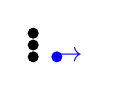
\begin{tikzpicture}
    \coordinate (11) at (0,0);
    \coordinate (12) at (0,0.15);
    \coordinate (13) at (0,0.3);
    \coordinate (14) at (0,0.45);
    \coordinate (21) at (0.15,0);
    \coordinate (22) at (0.15,0.15);
    \coordinate (23) at (0.15,0.3);
    \coordinate (31) at (0.3,0);
    \coordinate (32) at (0.3,0.15);
    \coordinate (41) at (0.45,0);
    \coordinate (51) at (0.6,0);
    \coordinate (61) at (0.75,0);
    \foreach \x in {(11),(12),(13)}{ \fill \x circle[radius=2pt]; }
    \foreach \x in {(31)}{\fill[blue] \x circle[radius=2pt]; }
    \node at (41) {\color{blue}$\rightarrow$};
  \end{tikzpicture}
  & $p^3(1-p)^2$ \\
  & 
  \begin{tikzpicture}
    \foreach \x in {(11),(12),(21)}{ \fill \x circle[radius=2pt]; }
    \foreach \x in {(41)}{\fill[blue] \x circle[radius=2pt]; }
    \node at (51) {\color{blue}$\rightarrow$};
  \end{tikzpicture}
  & $3p^3(1-p)^4$ \\
  & 
  \begin{tikzpicture}
    \foreach \x in {(11),(22),(21)}{ \fill \x circle[radius=2pt]; }
    \foreach \x in {(41)}{\fill[blue] \x circle[radius=2pt]; }
    \node at (51) {\color{blue}$\rightarrow$};
  \end{tikzpicture}
  & $3p^3(1-p)^5$ \\
  & 
  \begin{tikzpicture}
    \foreach \x in {(11),(21),(31)}{ \fill \x circle[radius=2pt]; }
    \foreach \x in {(51)}{\fill[blue] \x circle[radius=2pt]; }
    \node at (61) {\color{blue}$\rightarrow$};
  \end{tikzpicture}
  & $6p^3(1-p)^7$\\\hline
  $W_4\setminus W_3$ &
  \begin{tikzpicture}
    \foreach \x in {(21),(22),(23)}{ \fill \x circle[radius=2pt]; }
    \foreach \x in {(11)}{\fill[blue] \x circle[radius=2pt]; }
  \end{tikzpicture}
  & $p^4(1-p)^3$ 
  \\
  & 
  \begin{tikzpicture}
    \foreach \x in {(21),(22),(31)}{ \fill \x circle[radius=2pt]; }
    \foreach \x in {(11)}{\fill[blue] \x circle[radius=2pt]; }
  \end{tikzpicture}
  & $3p^4(1-p)^4$ \\
  & 
  \begin{tikzpicture}
    \foreach \x in {(21),(32),(31)}{ \fill \x circle[radius=2pt]; }
    \foreach \x in {(11)}{\fill[blue] \x circle[radius=2pt]; }
  \end{tikzpicture}
  & $3p^4(1-p)^5$ \\
  & 
  \begin{tikzpicture}
    \foreach \x in {(21),(31),(41)}{ \fill \x circle[radius=2pt]; }
    \foreach \x in {(11)}{\fill[blue] \x circle[radius=2pt]; }
  \end{tikzpicture}
  & $6p^4(1-p)^6$
  \\ &
  \begin{tikzpicture}
    \foreach \x in {(11),(12),(31)}{ \fill \x circle[radius=2pt]; }
    \foreach \x in {(21)}{\fill[blue] \x circle[radius=2pt]; }
  \end{tikzpicture}
  & $3p^4(1-p)^3$ \\
  & 
  \begin{tikzpicture}
    \foreach \x in {(11),(32),(31)}{ \fill \x circle[radius=2pt]; }
    \foreach \x in {(21)}{\fill[blue] \x circle[radius=2pt]; }
  \end{tikzpicture}
  & $3p^4(1-p)^5$ \\
  & 
  \begin{tikzpicture}
    \foreach \x in {(11),(31),(41)}{ \fill \x circle[radius=2pt]; }
    \foreach \x in {(21)}{\fill[blue] \x circle[radius=2pt]; }
  \end{tikzpicture}
  & $6p^4(1-p)^6$\\
  & 
  \begin{tikzpicture}
    \foreach \x in {(11),(21),(41)}{ \fill \x circle[radius=2pt]; }
    \foreach \x in {(31)}{\fill[blue] \x circle[radius=2pt]; }
  \end{tikzpicture}
  & $6p^4(1-p)^6$ \\ \hline
\end{tabular}

First:
\begin{align*}
  p^3(1-p)^2 & \geq 4p^4(1-p)^3,\\ 3p^3(1-p)^5 & \geq
  12p^4(1-p)^6,\\ 3p^3(1-p)^4 & + 6p^3(1-p)^7 - 3p^4(1-p)^4 - 6
  p^4(1-p)^5 - 6 p^4(1-p)^6 \\ & \geq
  6p^3(1-p)^6 (1  -2p) + 3p^3(1-p)^5 - 6p^4(1-p)^5 \geq 0
\end{align*}


Let us illustrate $p_4 - p_5$:

\begin{tabular}{l | l |l} \hline
  \vphantom{$\int$} $W_4\setminus W_5$& 
  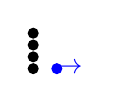
\begin{tikzpicture}
    \coordinate (11) at (0,0);
    \coordinate (12) at (0,0.15);
    \coordinate (13) at (0,0.3);
    \coordinate (14) at (0,0.45);
    \coordinate (21) at (0.15,0);
    \coordinate (22) at (0.15,0.15);
    \coordinate (23) at (0.15,0.3);
    \coordinate (24) at (0.15,0.45);
    \coordinate (31) at (0.3,0);
    \coordinate (32) at (0.3,0.15);
    \coordinate (33) at (0.3,0.3);
    \coordinate (41) at (0.45,0);
    \coordinate (42) at (0.45,0.15);
    \coordinate (51) at (0.6,0);
    \coordinate (61) at (0.75,0);
    \coordinate (71) at (0.9,0);
    \foreach \x in {(11),(12),(13),(14)}{ \fill \x circle[radius=2pt]; }
    \foreach \x in {(31)}{\fill[blue] \x circle[radius=2pt]; }
    \node at (41) {\color{blue}$\rightarrow$};
  \end{tikzpicture}
  & $p^4(1-p)^2$ \\
  &
  \begin{tikzpicture}
    \foreach \x in {(11),(12),(13),(21)}{ \fill \x circle[radius=2pt]; }
    \foreach \x in {(41)}{\fill[blue] \x circle[radius=2pt]; }
    \node at (51) {\color{blue}$\rightarrow$};
  \end{tikzpicture}
  & $4p^4(1-p)^4$ \\
  &
  \begin{tikzpicture}
    \foreach \x in {(11),(12),(21),(22)}{ \fill \x circle[radius=2pt]; }
    \foreach \x in {(41)}{\fill[blue] \x circle[radius=2pt]; }
    \node at (51) {\color{blue}$\rightarrow$};
  \end{tikzpicture}
  & $6p^4(1-p)^5$ \\
  & 
  \begin{tikzpicture}
    \foreach \x in {(11),(21),(22),(23)}{ \fill \x circle[radius=2pt]; }
    \foreach \x in {(41)}{\fill[blue] \x circle[radius=2pt]; }
    \node at (51) {\color{blue}$\rightarrow$};
  \end{tikzpicture}
  & $4p^4(1-p)^6$ \\
  & 
  \begin{tikzpicture}
    \foreach \x in {(11),(12),(21),(31)}{ \fill \x circle[radius=2pt]; }
    \foreach \x in {(51)}{\fill[blue] \x circle[radius=2pt]; }
    \node at (61) {\color{blue}$\rightarrow$};
  \end{tikzpicture}
  & $12p^4(1-p)^{7}$\\  & 
  \begin{tikzpicture}
    \foreach \x in {(11),(22),(21),(31)}{ \fill \x circle[radius=2pt]; }
    \foreach \x in {(51)}{\fill[blue] \x circle[radius=2pt]; }
    \node at (61) {\color{blue}$\rightarrow$};
  \end{tikzpicture}
  & $12p^4(1-p)^8$\\  & 
  \begin{tikzpicture}
    \foreach \x in {(11),(32),(21),(31)}{ \fill \x circle[radius=2pt]; }
    \foreach \x in {(51)}{\fill[blue] \x circle[radius=2pt]; }
    \node at (61) {\color{blue}$\rightarrow$};
  \end{tikzpicture}
  & $12p^4(1-p)^9$\\  & 
  \begin{tikzpicture}
    \foreach \x in {(11),(21),(31),(41)}{ \fill \x circle[radius=2pt]; }
    \foreach \x in {(61)}{\fill[blue] \x circle[radius=2pt]; }
    \node at (71) {\color{blue}$\rightarrow$};
  \end{tikzpicture}
  & $24p^4(1-p)^{11}$\\\hline
  $W_5\setminus W_4$ &
  \begin{tikzpicture}
    \foreach \x in {(21),(22),(23),(24)}{ \fill \x circle[radius=2pt]; }
    \foreach \x in {(11)}{\fill[blue] \x circle[radius=2pt]; }
  \end{tikzpicture}
  & $p^5(1-p)^4$ 
  \\
  & 
  \begin{tikzpicture}
    \foreach \x in {(21),(22),(23),(31)}{ \fill \x circle[radius=2pt]; }
    \foreach \x in {(11)}{\fill[blue] \x circle[radius=2pt]; }
  \end{tikzpicture}
  & $4p^5(1-p)^5$ \\
  & 
  \begin{tikzpicture}
    \foreach \x in {(11),(12),(13),(31)}{ \fill \x circle[radius=2pt]; }
    \foreach \x in {(21)}{\fill[blue] \x circle[radius=2pt]; }
  \end{tikzpicture}
  & $4p^5(1-p)^3$ \\
  & 
  \begin{tikzpicture}
    \foreach \x in {(21),(22),(31),(32)}{ \fill \x circle[radius=2pt]; }
    \foreach \x in {(11)}{\fill[blue] \x circle[radius=2pt]; }
  \end{tikzpicture}
  & $6p^5(1-p)^6$ \\
  & 
  \begin{tikzpicture}
    \foreach \x in {(11),(12),(31),(32)}{ \fill \x circle[radius=2pt]; }
    \foreach \x in {(21)}{\fill[blue] \x circle[radius=2pt]; }
  \end{tikzpicture}
  & $6p^5(1-p)^5$ \\
  & 
  \begin{tikzpicture}
    \foreach \x in {(21),(31),(32),(33)}{ \fill \x circle[radius=2pt]; }
    \foreach \x in {(11)}{\fill[blue] \x circle[radius=2pt]; }
  \end{tikzpicture}
  & $4p^5(1-p)^7$
  \\ &
  \begin{tikzpicture}
    \foreach \x in {(11),(31),(32),(33)}{ \fill \x circle[radius=2pt]; }
    \foreach \x in {(21)}{\fill[blue] \x circle[radius=2pt]; }
  \end{tikzpicture}
  & $6p^5(1-p)^7$
  \\ &
  \begin{tikzpicture}
    \foreach \x in {(21),(22),(31),(41)}{ \fill \x circle[radius=2pt]; }
    \foreach \x in {(11)}{\fill[blue] \x circle[radius=2pt]; }
  \end{tikzpicture}
  & $12p^5(1-p)^7$ \\
  & \begin{tikzpicture}
    \foreach \x in {(11),(12),(31),(41)}{ \fill \x circle[radius=2pt]; }
    \foreach \x in {(21)}{\fill[blue] \x circle[radius=2pt]; }
  \end{tikzpicture}
  & $12p^5(1-p)^6$ \\
  & \begin{tikzpicture}
    \foreach \x in {(11),(12),(21),(41)}{ \fill \x circle[radius=2pt]; }
    \foreach \x in {(31)}{\fill[blue] \x circle[radius=2pt]; }
  \end{tikzpicture}
  & $12p^5(1-p)^6$ \\
  & 
  \begin{tikzpicture}
    \foreach \x in {(21),(31),(32),(41)}{ \fill \x circle[radius=2pt]; }
    \foreach \x in {(11)}{\fill[blue] \x circle[radius=2pt]; }
  \end{tikzpicture}
  & $12p^5(1-p)^8$ \\
  & 
  \begin{tikzpicture}
    \foreach \x in {(11),(31),(32),(41)}{ \fill \x circle[radius=2pt]; }
    \foreach \x in {(21)}{\fill[blue] \x circle[radius=2pt]; }
  \end{tikzpicture}
  & $12p^5(1-p)^8$ \\
  & 
  \begin{tikzpicture}
    \foreach \x in {(11),(21),(22),(41)}{ \fill \x circle[radius=2pt]; }
    \foreach \x in {(31)}{\fill[blue] \x circle[radius=2pt]; }
  \end{tikzpicture}
  & $12p^5(1-p)^7$ \\
  & 
  \begin{tikzpicture}
    \foreach \x in {(21),(31),(41),(42)}{ \fill \x circle[radius=2pt]; }
    \foreach \x in {(11)}{\fill[blue] \x circle[radius=2pt]; }
  \end{tikzpicture}
  & $12p^5(1-p)^9$\\
  & 
  \begin{tikzpicture}
    \foreach \x in {(11),(31),(41),(42)}{ \fill \x circle[radius=2pt]; }
    \foreach \x in {(21)}{\fill[blue] \x circle[radius=2pt]; }
  \end{tikzpicture}
  & $12p^5(1-p)^9$\\
  & 
  \begin{tikzpicture}
    \foreach \x in {(11),(21),(41),(42)}{ \fill \x circle[radius=2pt]; }
    \foreach \x in {(31)}{\fill[blue] \x circle[radius=2pt]; }
  \end{tikzpicture}
  & $12p^5(1-p)^9$\\
  & 
  \begin{tikzpicture}
    \foreach \x in {(21),(31),(41),(51)}{ \fill \x circle[radius=2pt]; }
    \foreach \x in {(11)}{\fill[blue] \x circle[radius=2pt]; }
  \end{tikzpicture}
  & $24p^5(1-p)^{10}$ \\
    & 
  \begin{tikzpicture}
    \foreach \x in {(11),(31),(41),(51)}{ \fill \x circle[radius=2pt]; }
    \foreach \x in {(21)}{\fill[blue] \x circle[radius=2pt]; }
  \end{tikzpicture}
  & $24p^5(1-p)^{10}$ \\
    & 
  \begin{tikzpicture}
    \foreach \x in {(11),(21),(41),(51)}{ \fill \x circle[radius=2pt]; }
    \foreach \x in {(31)}{\fill[blue] \x circle[radius=2pt]; }
  \end{tikzpicture}
  & $24p^5(1-p)^{10}$ \\
    & 
  \begin{tikzpicture}
    \foreach \x in {(11),(21),(31),(51)}{ \fill \x circle[radius=2pt]; }
    \foreach \x in {(41)}{\fill[blue] \x circle[radius=2pt]; }
  \end{tikzpicture}
  & $24p^5(1-p)^{10}$ \\
  \hline
\end{tabular}

$$ \frac d{dp} p(1-p)^k = (1-p)^k - kp(1-p)^{k-1} = (1-p)^{k-1}(1-p(k+1)),$$
so
$$ \frac{(k+1)^{k+1}}{k^k} p(1-p)^k \leq 1.$$ $n$ case probability

  \begin{tikzpicture}
    \coordinate (11) at (0,0);
    \coordinate (12) at (0,0.15);
    \coordinate (21) at (0.15,0);
    \coordinate (22) at (0.15,0.15);
    \coordinate (31) at (.3,0);
    \coordinate (32) at (.3,0.15);
    \foreach \x in {(11), (12), (21), (31), (32)}{ \fill \x circle[radius=2pt]; }
\end{tikzpicture}


With $p_0=1$, 
\begin{align*}
  p_n & = \sum_{k=0}^{n-1} \binom n k (1-p)^k p^{n-k}
  p_k.\\ \sum_{n=1}^\infty p_ns^n & = \sum_{k=0}^\infty
  \sum_{n=k+1}^\infty \binom n k (1-p)^kp^{n-k} p_k s^n \\ & =
  \sum_{k=0}^\infty \frac{1}{k!} ((1-p)s)^k p_k \sum_{n=k+1}^\infty
  n\cdots (n-k+1) (ps)^{n-k} \\ & = \sum_{k=0}^\infty \frac{1}{k!}
  ((1-p)s)^k p_k \frac{d^k}{dx^k} \sum_{n=1}^\infty x^n \Big|_{x = ps}
  \\ & = \sum_{k=0}^\infty \frac{1}{k!} ((1-p)s)^k p_k \frac{d^k}{dx^k}
  \Big( \frac{1}{1-x} - 1\Big) \Big|_{x = ps} \\ & = \frac{ps}{1-ps} +
  \sum_{k=1}^\infty \frac{1}{k!} ((1-p)s)^k p_k (-1)^k k! (1-ps)^{-(k+1)}
  \\ & = \frac{ps}{1-ps} - \frac{1}{1-ps} \sum_{k=1}^\infty
  p_k \Big(\frac{-(1-p)s}{1 - ps}\Big)^k
\end{align*}

Note that 
\begin{align*}
  \mathbf P(\max_{i=1,...,n} T_i \leq t - \log_{1-p} n ) & = (1 -
  (1-p)^{t - \log_{1-p} n})^n \approx \exp( - (1-p)^t), \\ \mathbf
  P(\max_{i=1,...,n} T_i = \lfloor t - \log_{1-p} n \rfloor) & \approx
  \exp( - (1-p)^t) - \exp( - (1-p)^{t-1}),\\ \mathbf P\Big(
  \bigcup_{i=1}^n \{T_i = a - \log_{1-p} n\}\Big) & = 1 -
  \prod_{i=1}^n \Big( 1 - (1-p)^{a- \log_{1-p} n - 1} p \Big) = 1 -
  \Big( 1 - (1-p)^{a- 1} p/n \Big)^n \\ & \approx 1 - \exp\Big(-
  (1-p)^{a- 1} p \Big) \\ p_n & \approx \sum_{t=-\infty}^\infty
  \big(\exp( - (1-p)^t) - \exp( - (1-p)^{t-1})\big)
  \prod_{a=-\infty}^{t-1} \Big( 1 - \exp\Big(-
  (1-p)^{a- 1} p \Big)\Big)
\end{align*}

$X \sim \exp(1)$, so
$$ \mathbf P(ts\leq X\leq (t+1)s) = e^{-ts} - e^{-(t+1)s} = e^{-ts}(1
- e^{-s}).$$

For $Z := \max_{i=1,...,n} X_i$,
\begin{align*}
  \mathbf P(Z \in dz) & = \frac{d}{dz} (1 - e^{-z})^n = n e^{-z}(1 -
  e^{-z})^{n-1}, \\ \mathbf P(Z - \lfloor Z\rfloor < x) & =
  \sum_{k=0}^\infty \int_k^{k+x} n e^{-z}(1 - e^{-z})^{n-1} dz =
  \sum_{k=0}^\infty (1 - e^{-z})^n\big|_{z=k}^{z=k+x} \\ & =
  \sum_{k=0}^\infty (1 - e^{-(k+x)})^n - (1 - e^{-k})^n
  \\ & = \sum_{k=0}^\infty (1 + e^{-x})^n (1 - e^{-k})^n + - (1 - e^{-k})^n
\end{align*}

For large $n$,
\begin{align*}
  p_n  := & \sum_t \mathbf P(\text{success}, \max_{i=1,...,n} T_i = t)
  \\ \approx & \sum_t \mathbf P(\bigcap_k \bigcup_i 1_{T_i = t-k},
  \max_{i=1,...,n} T_i = t)
\end{align*}

Heuristics with $p = 1 - e^{-s}$, so $1-p = e^{-s}$
$$ p_ \infty \approx \prod_{k=1}^\infty (1 - e^{-ks}) =
\prod_{k=1}^\infty (1 - (1-p)^{k})$$

\begin{align*}
  a_1 & = 1,
  \\ a_2 & = p + (1-p)p ,\\
  a_3 & = p^2 + p^2(1-p) + (1-p)^2 a_2
  p_n & \approx p^2 + 2p(1-p)p + (1-p)^2
\end{align*}


Here is another probabilsitic model capturing the model: Take
$X_1,...,X_n \sim \exp(1)$ independently, and independent Poisson
processes $P_1,...,P_n$ with rate $\lambda>0$ with $p = 1/(1+\lambda)$
or $\lambda = (1-p)/p$. Then, by construction, $T_i = |\{t \leq X_i:
t\in P_i\}| \sim geo(p)$. Rather, let us assume that there is a single
Poisson process $P$, which makes the resulting geometric RVs
dependent. Then we want to compute the probability that between any
two clicks of $P$ there is at least one $i$ such that $X_i$ runs
off. This can be computed via
$$ \prod_{k=1}^n \frac{k}{k + \lambda}.$$

Let $p_{n,t}$ be the probability of a win when starting with $n$
coins after exactly $t$ coin tosses. Then,
$$ p_{n+1,t} = p_{n,t}(1 - (1-p)^t) + p_{n, t-1}(1-p)^{t-1} p$$ So,
with $a_n(s) = \sum_t p_{n,t} s^t$,
\begin{align*}
  a_{n+1}(s) & = \sum_t p_{n+1,t}s^t = a_n(s) - a_n(s(1-p)) + sp
  a_{n}(s(1-p)) = a_n(s) - a_n(s(1-p))(1 - sp)
\end{align*}
$$ P(S_{n+1} | \mathcal F_n) = 1_{S_n} ( 1 - (1-p)^{T_n+1})$$
\begin{align*}
  \mathbf E[A_n1_{S_{n+1}} | \mathcal F_n] = A_n 1_{S_n} (1 -
    (1-p)^{T_n+1}) = A_{n-1} 1_{S_n}
\end{align*}
So, $A_n = \prod_{k=1}^n (1 - (1-p)^{T_k+1})$

\newpage

For the case $p<1/2$ we have the following:

\begin{lemma}
  Let $p<1/2$. If $w_{n-1,p} = \max_{k=1,...,n-1} w_{k,p}$. Then,
  $w_{n,p} < w_{n-1,p}$.
\end{lemma}

\begin{proof}
  First, note that (since $p < 1/2$),
  $$ n \mapsto \frac{p^n}{(1-p)^n + p^n} = \frac{1}{1 + ((1-p)/p)^n}
  \text{ is decreasing},$$ in particular $\frac{p^n}{(1-p)^n + p^n} <
  p = w_{1,p}$. From here on, we copy the calculations from
  Lemma~\ref{l1}: We compute
  \begin{align*}
    w_{n,p} & = p^n + \sum_{j=1}^{n-1} \binom n j p^{n-j} (1-p)^j
    w_{n-1,p} \\ & = p^n + (1 - p^n - (1-p)^n)w_{n-1,p} = w_{n-1,p} +
    p^n(1 - w_{n-1,p}) - (1-p)^n w_{n-1,p}.
  \end{align*}
  Clearly, we have $w_{n,p} < w_{n-1,p}$ iff
  \begin{align*}
    \frac{(1-p)^n}{p^n} > \frac{1 - w_{n-1,p}}{w_{n-1,p}} =
    \frac{1}{w_{n-1,p}} - 1, \quad \text{ i.e. } \quad w_{n-1,p} >
    \frac{p^n}{(1-p)^n + p^n}.
  \end{align*}
  The latter holds since $w_{n-1,p} \geq w_{1,p} = p >
  \frac{p^n}{(1-p)^n + p^n}$.
\end{proof}

\newpage


Let us study the case $p<1/2$. Setting $v_0 := 1$, note that
\eqref{eq:wn} changes to
\begin{equation}\label{eq:wn1}
  \begin{aligned}
    v_{n,p} & = \sum_{j=0}^{n-1} \binom n j p^{n-j} (1-p)^j v_j \\ & =
    \sum_{j=0}^{n-1} \Big(\binom {n-1}{j} +
    \binom{n-1}{j-1}\Big)p^{n-j} (1-p)^j v_j \\ & = p v_{n-1}(1 +
    (1-p)^{n-1}) + \sum_{j=0}^{n-2} \binom{n-1}{j}
    p^{n-1-j}(1-p)^{j+1} (v_j + v_{j+1} - v_j) \\ & = v_{n-1} +
    p(1-p)^{n-1} v_{n-1} + (1-p)\sum_{j=0}^{n-2} \binom{n-1}{j}
    p^{n-1-j}(1-p)^{j} (v_{j+1} - v_j) \\
    & = v_{n-1} +
    p(1-p)^{n-1} v_{n-1} - (1-p)^{n}(v_n - v_{n-1}) + (1-p)\sum_{j=0}^{n-1} \binom{n-1}{j}
    p^{n-1-j}(1-p)^{j} (v_{j+1} - v_j) 
  \end{aligned}
\end{equation}
So, we find that
$$ v_n < v_{n-1} \quad \iff \quad p(1-p)^{n-1} v_{n-1} <
(1-p)\sum_{j=0}^{n-2} \binom{n-1}{j} p^{n-1-j}(1-p)^{j} (v_{j} -
v_{j+1}) $$
With
\begin{align*}
  \sum_{j=0}^{n-1} & \binom{n}{j} p^{n-j}(1-p)^{j} (v_{j+1} - v_j)
  \\ & = \sum_{j=1}^{n} \Big(\binom{n-1}{j-1} +
  \binom{n-1}{j-2}\Big)p^{n-j+1}(1-p)^{j-1} v_j - \sum_{j=0}^{n-1}
  \Big(\binom{n-1}{j-1} + \binom{n-1}{j}\Big) p^{n-j}(1-p)^{j} v_j
  \\ & = (1-p)^n v_n + (2p-1) \sum_{j=1}^{n} \binom{n-1}{j-1}
  p^{n-j}(1-p)^{j-1} v_j \\ & + \sum_{j=0}^{n-2}
  \binom{n-1}{j}p^{n-j-1}(1-p)^{j+1} v_{j+2} - \sum_{j=0}^{n-1}
  \binom{n-1}{j}p^{n-j}(1-p)^{j} v_{j}
\end{align*}

Note that
\begin{align*}
  \sum_{j=i+1}^{n-1} \binom{n}{j} \binom{j}{i} (1-p)^{j-i} & =
  \frac{n!}{i!(n-i)!} \sum_{j=i+1}^{n-1} \binom{n-i}{j - i}
  (1-p)^{j-i} \\ & = \binom{n}i \sum_{j=1}^{n-i-1} \binom{n-i}{j}
  (1-p)^j \\ & = \binom{n}i \big((2-p)^{n-i} - 1 - (1-p)^{n-i}\big)
\end{align*}

Pluggin in this result for $v_{j+1} - v_j$, we obtain
\begin{equation}\label{eq:wn1}
  \begin{aligned}
    v_{n,p} - v_{n-1} & = p(1-p)^{n-1} v_{n-1} + (1-p)
    \sum_{j=0}^{n-2} \binom{n-1}{j} p^{n-1-j}(1-p)^{j} \\ & \qquad
    \qquad \qquad \qquad \cdot \Big(p(1-p)^jv_j + (1-p)
    \sum_{i=0}^{j-1} \binom{j}{i} p^{j-i}(1-p)^i (v_{i+1} - v_i)\Big)
    \\ & = p(1-p)^{n-1} v_{n-1} + (1-p) \sum_{j=0}^{n-2}
    \binom{n-1}{j} p^{n-1-j}(1-p)^{j} p(1-p)^jv_j \\ & + (1-p)^2
    \sum_{i=0}^{n-3} p^{n-1-i} (1-p)^i (v_{i+1} - v_i)
    \underbrace{\sum_{j=i+1}^{n-2} \binom{n-1}{j} \binom{j}{i} (1-p)^j}_{= \frac{(n-1)!}{i!(n-1-i)!} \sum_{j=i+1}^{n-2} \binom{n-1-i}{j - i} (1-p)^j}
  \end{aligned}
\end{equation}
Let (with $x_n = v_{n+1} - v_n$),
\begin{align*}
  x_{n} & = a_{n} + (1-p)\sum_{j=0}^{n-1} \binom{n}{j}p^{n-j}(1-p)^{j}x_j,
\end{align*}
then, with
\begin{align*}
  \sum_{j=k+1}^{n-1} \binom{n}{j}\binom j k (1-p)^{j} & =
  \frac{n!}{k!(n-k)!} \sum_{j=k+1}^{n-1} \frac{(n-k)!}{(n-j)!(j-k)!}
  (1-p)^{j} = \binom n k \sum_{j=k+1}^{n-1} \binom{n-k}{j-k} (1-p)^{j}
  \\ & = \binom n k (1-p)^k \sum_{j=1}^{n-k-1} \binom{n-k}{j}
  (1-p)^{j} \\ & = \binom n k (1-p)^k \Big((2-p)^{n-k} - 1 -
  (1-p)^{n-k} \Big)
\end{align*}
we have
\begin{align*}
  x_n & = a_{n} + (1-p)\sum_{j=0}^{n-1} \binom{n}{j}p^{n-j}(1-p)^{j}
  \Big(a_j + (1-p)\sum_{k=0}^{j-1} \binom j k p^{j-k-1} (1-p)^k
  x_k\Big) \\ & = a_{n} + (1-p)\sum_{j=0}^{n-1}
  \binom{n}{j}p^{n-j}(1-p)^{j} a_j + (1-p)^2\sum_{k=0}^{n-2}(1-p)^k p^{n-k-1}
  x_k \sum_{j=k+1}^{n-1} \binom{n}{j}\binom j k (1-p)^{j}  \Big)
  \\ & =
\end{align*}



We have
\begin{align*}
  w_{1,p} & = p,\\ w_{2,p} & = p^2 + 2p^2(1-p) = p^2(3-2p) = p
  (3p-2p^2) < p = w_{1,p},\\ w_{3,p} & = p^3 + 3p(1-p)(p w_{1,p} +
  (1-p) w_{2,p}) = p^3(1 + 3(1-p)(1 + (1-p)(3-2p))) \\ & = p^3(1 +
  3(1-p)(4 -5p + 2p^2)) = p^3(13 -27p -21p^2 - 6p^3),\\ w_{3,p} & <
  p^3 + 3p(1-p)p = p^2(3-2p) = w_{2,p}, \\ w_{4,p} & = p^4 +
  4p^3(1-p)w_{1,p} + 6p^2(1-p)^2w_{2,p} + 4p(1-p)^3 w_{3,p}
\end{align*}

\begin{align*}
  w_{2,p} & = p^2 + 2p(1-p)w_{1,p} \\ w_{3,p} & = p^3 + 3p^2(1-p)
  w_{1,p} + 3p(1-p)^2 w_{2,p} \\ & \leq p^3 + p^2(1-p)w_{1,p} +
  p(1-p)^2 w_{1,p} + 2p(1-p) w_{1,p} \\ & = (p + p(1-p) + (1-p)^2)
  )p^2 + 2p(1-p) w_{1,p} = w_{2,p} \\ w_{4,p} & = p^4 +
  4p^3(1-p)w_{1,p} + 6p^2(1-p)^2w_{2,p} + 4p(1-p)^3 w_{3,p} \\ & \leq
  p^4 + 4p^3(1-p)w_{1,p} + 3p^2(1-p)^2w_{1,p} + p(1-p)^3 w_{2,p} +
  3p(1-p)^2w_{2,p} \\ & \leq p^4 + p^3(1-p)w_{1,p} + p(1-p)^3 w_{2,p}
  + 3p^2(1-p)w_{1,p} + 3p(1-p)^2w_{2,p} \\ & = p^2(p^2 + p^2(1-p) +
  (1-p)^3) - p(1-p)^3p(1-2p)(1-p) + 3p^2(1-p) w_{1,p} + 3p(1-p)^2w_{2,p} \\ w_{4,p} & = p^4 +
  4p^3(1-p)w_{1,p} + 6p^2(1-p)^2w_{2,p} + 4p(1-p)^3 w_{3,p} \\ & \leq
  p^3(p + p(1-p) + (1-p)^2) + 3p^3(1-p)w_{1,p} + 3p^2(1-p)^2w_{1,p}(p
  + p(1-p) + (1-p)^2)w_{1,p} + 3p(1-p)^2 w_{2,p} \\ & \leq p^3 +
  3p^2(1-p)w_{1,p} - 3p^2(1-p)^2 w_{1,p} + 5p^2(1-p)^2w_{2,p} +
  4p(1-p)^3 w_{2,p} \\ & = p^3 + p(1-p)w_{1,p}(3p^2 + 2p(1-p) +
  (1-p)^2) + 3p(1-p)^2 w_{2,p}
\end{align*}

We have $w_{n} - w_{n+1} = a_n - b_n$, where $a_0 = 1-p, b_0=0$,
\begin{align*}
  a_n & = (1-p)\sum_{j=0}^{n-1}\binom{n}{j}p^{n-j}(1-p)^{j} a_j,\\
  b_n & = p(1-p)^{n}w_{n} + (1-p)\sum_{j=1}^{n-1}\binom{n}{j}p^{n-j}(1-p)^{j}b_j
\end{align*}

For small $p$,
\begin{align*}
  w_{1,p} & = p,\\ w_{2,p} & \approx 3p^2,\\ w_{3,p} & \approx 13p^3,
  \\ w_{4,p} & \approx 85p^4 \\ a_n & = \sum_{j=0}^{n-1}\binom nj a_j
\end{align*}

Is $n\mapsto w_{n,p}$ decreasing for some $p$?

Let us try to prove that $w_{n-1,p} - w_{n,p} \geq Cp(1-p)^{n-1}$ for
some $C$.

\begin{align*}
  w_0 - w_1 & = 1-p,\\ w_1 - w_2 & = - p(1-p)w_1 + p(1-p)(w_0-w_1) =
  p(1-p)(w_0 - 2w_1),\\ w_2 & = p(1 - (1-p)(1-2p)),\\ 1 - w_2 & = w_0
  - w_1 + w_1 - w_2 = (1 + p(1-2p))(w_0 - w_1)\\ w_2 - w_3 & =
  3p(1-p)^2 (w_1 - w_2), \\ w_2 - w_3 & = -p(1-p)^2 w_2 +
  p^2(1-p)(1-w_1) + 2 p (1-p)^2 (w_1 - w_2)\\ w_1 - w_2 & = p(1 - 3p +
  2p^2) = p(1-2p)(1-p) = p(1-2p)(w_0 - w_1),\\ w_2 - w_3 & = 3p(1-p)^2
  (w_1 - w_2),\\ w_3 & = w_2 - 3p(1-p)^2 (w_1 - w_2),\\ w_3 - w_4 & =
  -p(1-p)^3 w_3 + (1-p)(p^3(w_0 - w_1) + 3p^2(1-p)(w_1 - w_2) +
  3p(1-p)^2(w_2 - w_3))
\end{align*}

For $n=2,3,...$,
\begin{align*}
  w_{n-1,p} - w_{n,p} & = \sum_{j=0}^{n-2} \binom {n-1} j
  p^{n-1-j}(1-p)^j w_{j,p} - \sum_{j=0}^{n-1} \Big(\binom {n-1} j +
  \binom {n-1} {j-1}\Big) p^{n-j}(1-p)^j w_{j,p} \\ & =
  \Big(\sum_{j=0}^{n-2} \binom {n-1} j
  p^{n-1-j}(1-p)^{j+1}w_{j,p}\Big) - p(1-p)^{n-1}w_{n-1,p} \\ & \qquad
  \qquad \qquad \qquad - \sum_{j=0}^{n-2}\binom{n-1}{j}
  p^{n-j-1}(1-p)^{j+1} w_{j+1,p} \\ & = - p(1-p)^{n-1} w_{n-1,p} +
  \sum_{j=0}^{n-2} \binom{n-1}{j} p^{n-1-j}(1-p)^{j+1}(w_{j,p} -
  w_{j+1,p}) \\ & = p(1-p)(\underbrace{p^{n-2}(1 - p) - (1-p)^{n-2}
    w_{n-1}}_{= \sum_{j=1}^{n-2} (1-p)^j p^{n-1-j}(w_j - w_{j+1})}) +
  \sum_{j=1}^{n-2} \binom{n-1}{j} p^{n-1-j}(1-p)^{j+1}(w_j - w_{j+1})
  \\& = - p^n + \sum_{k=0}^{n-2} p^{n-k}(1-p)^k w_k -
  p^{n-1-k}(1-p)^{k+1}w_{k+1} + \sum_{j=0}^{n-2} \binom{n-1}{j}
  p^{n-1-j}(1-p)^{j+1}(w_{j,p} - w_{j+1,p}) \\ & \geq -
  p(1-p)^{n-1}w_{n-1,p} + C p \sum_{j=1}^{n-2} \binom{n-1}{j}
  p^{n-1-j}(1-p)^{2j} \\ & = - p(1-p)^{n-1}w_{n-1,p} + C p (1 - p +
  p^2)^{n-1} - Cp (1-p)^{2n-2}
\end{align*}
so $w_{n-1,p} > w_{n,p}$ if $w_{n-1,p} < \frac{p^{n-2}}{(1-p)^{n-3}}$.

\newpage

\section{A version of the game in continuous time}
Consider a Poisson process at rate $x$, as well as $X_1,...,X_n \sim
\exp(1)$, which are independent. Then, we are asking for the
probability that no two points $T_k, T_{k+1}$ of the $x$-Poisson
process happen with $X_1,...,X_n \notin \{T_k, T_{k+1}\}$ and $X_i >
T_{k+1}$ for at least one $i$. Again, call this probability $w_n$. We
obtain the recursion, with $w_0=1$,
$$ w_n = \sum_{k=0}^{n-1} \frac{n\cdots (k+1) \cdot x}{(n+x)\cdots
  (k+1+x)(k+x)} w_k = x \sum_{k=0}^{n-1}
\frac{\Gamma(n+1)\Gamma(k+1+x)}{\Gamma(k+2)\Gamma(n+1+x)} w_k.$$
  Note that for $x=1$,
$$ w_n = \frac{1}{n+1} \sum_{k=0}^{n-1} w_k = \frac{1}{n+1} \Big(1 +
  \sum_{k=1}^{n-1} w_k\Big), $$ which is solved by $w_1 = w_2 = ... =
  \tfrac 12$. Recursively, using the recursion for $w_{n-1}$ in the
  fourth equality,
\begin{align*}
w_n - w_{n-1} & = \sum_{k=0}^{n-1} \frac{n\cdots (k+1) \cdot
  x}{(n+x)\cdots (k+1+x)(k+x)} w_k - \sum_{k=0}^{n-2}
\frac{(n-1)\cdots (k+1) \cdot x}{(n-1+x)\cdots (k+1+x)(k+x)} w_k \\ &
= \frac{nx}{(n+x)(n-1+x)}w_{n-1} + \sum_{k=0}^{n-2}\Big(\frac{n\cdots
  (k+1) \cdot x - (n+x)(n-1)\cdots (k+1) \cdot x}{(n+x)\cdots
  (k+1+x)(k+x)}w_k \\ & = \frac{nx}{(n+x)(n-1+x)}w_{n-1} - x^2
\sum_{k=0}^{n-2} \frac{(n-1)\cdots (k+1)}{(n+x)\cdots (k+1+x)(k+x)}w_k
\\ & =\frac{nx}{(n+x)(n-1+x)}w_{n-1} - \frac{x}{n+x} w_{n-1} =
\frac{x}{n+x} \Big(\frac{n}{n-1+x} - 1\Big)w_{n-1}.
\end{align*}
From the last line, it is clear that
$$w_n - w_{n-1} < 0 \quad \iff \quad x>1. $$
In particular, $n\mapsto w_n$ is decreasing for $x>1$.

\end{document}
\newpage


Let us compute some bounds. Starting with $n$ coins, we might in the
first round set aside a single coin, and afterwards play
optimally. This gives us
\begin{align*}
  w_{n,p} & \leq (1-p)^n + (1 - p^n)w_{n-1,p},\\ w_{n,p} - w_{n-1,p} &
  \leq (1-p)^n - p^n w_{n-1,p},\\ w_{n,p} & \leq
  \sum_{k=0}^{n-1}(1-p)^{k+1} - p^{k+1} w_{k,p} = \frac{1 -
    (1-p)^n}{p} - \sum_{k=0}^{n-1} p^{k+1} w_{k,p}.
\end{align*}
Applying the discrete Gronwall inequality gives
\begin{align*}
w_{n,p} & \leq \frac{1 - (1-p)^n}{p} + \sum_{k=0}^{n-1}\frac{1 -
  (1-p)^k}{p} p^{k+1} \exp\Big( - \sum_{j=k+1}^{n-1} p^{j+1} \Big)
\end{align*}


Let us compute the first few values. Note that for $n=1,2$, there is
literally no choice. For $n=1$, set aside the head if possible. For
$n=2$, set aside one coin unless both come up heads, in which case you
set aside both coins. For $n=3$, if there are 0~or~1 coin, set aside
one coin. If all are heads, set aside all three. However, if there are
two heads, the first decision has to be made: With $w_{0,p}=0$,
\begin{align*}
  w_{1,p} & = 1-p,\\ w_{2,p} & = (2-p)(1-p)^2 + 2p(1-p)(1-p) =
  (2+p)(1-p)^2,\\ w_{3,p} & = (w_{2,p} + 1)(1-p)^3 + 3p^2(1-p)
  (w_{1,p} \wedge w_{2,p}) + 3p(1-p)^2 w_{2,p}, \\w_{4,p} & = (w_{3,p}
  + 1)(1-p)^4 + 4p^3(1-p) (w_{1,p} \wedge w_{2,p}\wedge w_{3,p})
  +6p^2(1-p)^2 (w_{2,p}\wedge w_{3,p}) + 4p(1-p)^3 w_{3,p}.
\end{align*}
Let us analyse $w_{3,p}$: We see that there is a distinction whether
$w_{1,p} < w_{2,p}$, i.e.\ $1 < (2+p)(1-p) = 2 -p - p^2$, i.e.\ $p <
\frac{\sqrt 5 + 1}{2} \approx 0.618 $. If $p < \frac{\sqrt 5 + 1}{2}$,
if two out of three coins come up heads, we set aside both of them,
whereas for $p > \frac{\sqrt 5 + 1}{2}$, we set aside only one.
\\ Using the same approach, let us analyse $w_{4,p}$. Here, we need to
understand when $w_{2,p} < w_{3,p}$. We distinguish two cases from
above: \\ $p > \frac{\sqrt 5 + 1}{2}$ (or $w_{2,p} < 1-p$). We already
know $w_{1,p} > w_{2,p}$. Hence,
$$ w_{3,p} = (1-p)^3 + (1-p^3)w_{2,p}. $$ From this, we see that
$w_{3,p} < w_{2,p}$ iff $(1-p)^3 - p^3 w_{2,p} = (1-p)^2((1-p) -
p^3(2+p)) < 0$, which is always true in this case and we have $w_{3,p}
< w_{2,p} < w_{1,p}$.\\
$p < \frac{\sqrt 5 + 1}{2}$ (or $w_{2,p} > 1-p$). Here, we get
$$ w_{3,p} = (1-p)^3 + 3p^2(1-p)^2 + ((1-p)^3 + 3p(1-p))w_{2,p}.$$


Let us try to show $w_{n,p} \leq w_{n-1,p}$ be induction. Assume this
inequality holds for all $k$ up to $n-1$. Then,
\begin{align*}
  w_{n,p} & = (w_{n-1,p} + 1) (1-p)^n + \sum_{j=1}^{n-1} \binom n j
  p^{n-j} (1-p)^{j} w_{n-1,p} \\ & = (1-p)^n + (1 - p^n) w_{n-1,p}
  \geq (1-p)^n + (1 - p^n) \frac{(1-p)^{n-1}}{p^{n-1}} =
  \frac{(1-p)^{n}}{p^n} \big(p^n + (p + p^2 + \cdots p^{n-1})\big),
\end{align*}
which is at most $w_{n-1,p}$ iff $(1-p)^n \leq p^n w_{n-1,p}$.



Let us consider the strategy of always setting aside as much heads as
possible. Here,
\begin{align*}
  \mathbb E[Z_n | \mathcal F_{n-1}] & = (Z_{n-1} + 1)(1-p)^n +
  \sum_{j=0}^{n-1} \binom n j p^{n-j}(1-p)^{j} Z_j \\ & = (1-p)^n +
  ((1-p)^n + np(1-p)^{n-1})Z_{n-1} + \sum_{j=0}^{n-2} \binom n j
  p^{n-j}(1-p)^{j} Z_j.
\end{align*}
Hence, with $a_{n,n} = 1$ for all $n$, 
\begin{align*}
  \mathbb E\Big[ \sum_{k=0}^n a_{kn} Z_k | \mathcal F_{n-1}] & =
  (1-p)^n + (a_{n-1,n} + ((1-p)^n + np(1-p)^{n-1}))Z_{n-1} +
  \sum_{k=0}^{n-2} (a_{kn} + \binom n k p^{n-k}(1-p)^k) Z_k
  \\ & \stackrel ! = \sum_{k=0}^{n-1} a_{k,n-1} Z_k.
\end{align*}
We find
\begin{align*}
  1 & = a_{n-1,n} + ((1-p)^n + np(1-p)^{n-1}),\\ a_{k,n-1} & = a_{kn}
  + \binom n k p^{n-k}(1-p)^k, \qquad k=0,...,n-2
\end{align*}

Let $J \sim B(n, 1-p)$. Then,
$$ Z_n = 1_{J = n} (1 + Z_{n-1}) + 1_{J < n} Z_{J} = Z_{J} - 1_{J = n} (Z_n - Z_{n-1} - 1) = Z_{J}$$
So, with $Z_0=0$, 
\begin{align*}
  \mathbb E[Z_1] & = (1-p), \\
  \mathbb E[Z_2] & = (1-p)^2 (1 + 1-p) + 2p(1-p)^2 = (1-p)^2 + (1-p)^2 (1 + p) = (1-p)^2 + (1-p)(1-p^2), \\
  \mathbb E[Z_3] & = (1-p)^3 + ((1-p)^3 + 3p(1-p)^2)((1-p)^2 + (1-p)(1-p^2)) + 3(1-p) p^2 (1-p) 
\end{align*}


Specifically, the test statistic, hereafter referred to as Delta
Likelihood, represents the difference in the likelihood of the
ancestry vector $\widehat q^K$ estimated for a given genotype if drawn
from any combination of the allele frequencies $(p)$ represented among
the $K=5$ reference groups minus the likelihood of the ancestry vector
$\widehat q^L$ estimated strictly from allele frequencies among the
$L=4$ domestic pig reference groups. Accordingly, if $p_{km}$ is the
frequency of the reference allele at locus $m$ in the $k$th pig
reference group, and $X_m = \{0,1,2\}$ is the number of reference
allele the individual under consideration carries, the Delta
Likelihood statistic for this individual can be calculated as:
\begin{align*}
  \Delta\ell(p|X) := \frac{1}{2M} \sum_{m=1}^M X_m \log \Big(
  \frac{\langle \widehat q^K, p_{\cdot m}\rangle}{\langle \widehat
    q^L, p_{\cdot m}\rangle} \Big) + (2 - X_m)
  \log\Big(\frac{1-\langle \widehat q^K, p_{\cdot m}\rangle}{1-\langle
    \widehat q^L, p_{\cdot m}\rangle}\Big).
\end{align*}
Here, $\langle q, p_{\cdot m}\rangle := \sum_{k=1}^K q_k p_{km}$ is
the probability of obtaining the reference allele for an individual
with admixture $q$ at locus $m$. Note that we assume that all loci are
bi-allelic; see Pfaffelhuber \& Rohde (2023) for a deeper analysis of
this likelihood and methods to compute $\widehat q^K$ and $\widehat
q^L$.

\vspace{2cm} For a bi-allelic marker with frequency $p_k$ in reference
group $k$, one can compute $\bar p := \frac{1}{K}(p_1 + \cdots + p_K)$
as well as $\overline{p(1-p)} := \frac{1}{K}(p_1(1-p_1) + \cdots +
p_K(1-p_K))$. Then, $F_{ST}$ is given by
$$ F_{ST} = \frac{\bar p(1-\bar p) - \overline{p(1-p)}}{\bar p(1-\bar
  p)}$$ for this marker. In general, high $F_{ST}$ means that allele
frequencies in the groups differ.
\end{document}








\thispagestyle{empty}

\author{\sc by A. Depperschmidt, A. Greven and P. Pfaffelhuber}

\date{\today}

%\vspace*{-5ex}

\maketitle

\noindent
In this note, we consider the tree-valued Fleming-Viot dynamics,
$(\mathcal U_t)_{t\geq 0}$. In the first section, we study the case
without types, mutation and selection. We answer the question raised
in [GPW10] and show that the mm-space does not have any atom for all
$t$, almost surely. In the second section, we study the case with
types by adding mutation, as studied in [DGP10]. Here, we show that,
for almost all $t$, the mmm-space admits a mark function.

\section{Auxiliary material}
\begin{lemma}\label{l1}
  For $\lambda,\lambda'\geq 0$, let
  \begin{equation}
    \label{eq:321}
    \begin{aligned}
      f_\lambda(t) & := \mathbf E[\langle \nu^{\mathcal U_t}, e^{-\lambda r_{12}}\rangle],\\
      \qquad g_{\lambda,\lambda'}(t) & := \mathbf E[\langle
      \nu^{\mathcal U_t}, e^{-\lambda r_{12} + \lambda'
        r_{13})}\rangle],\\
      h_{\lambda, \lambda'}(t) & := \mathbf E[\langle \nu^{\mathcal
        U_t}, e^{-\lambda r_{12} + \lambda'r_{34})}\rangle].
    \end{aligned}
  \end{equation}
  Then, for all $t>0$, there is a constant $c$ which is independent of
  $\lambda, \lambda'$ and $t$ such that
  \begin{equation}
    \label{eq:322}
    \begin{aligned}
      f_\lambda(t) - f_\lambda(\infty) & = e^{-\lambda
        t}\big(f_\lambda(0) - f_\lambda(\infty)\big),\\
      \Big|g_{\lambda,\lambda'}(t) -g_{\lambda,\lambda}(\infty)\Big|&
      \leq e^{-c(\lambda\wedge\lambda')t}\big|g_{\lambda,\lambda'}(0)
      -
      g_{\lambda,\lambda'}(\infty) \big|\\
      \Big|h_{\lambda,\lambda'}(t) -h_{\lambda,\lambda}(\infty)\Big|&
      \leq e^{-c(\lambda\wedge\lambda')t}\big|h_{\lambda,\lambda'}(0)
      - h_{\lambda,\lambda'}(\infty) \big|
    \end{aligned}
  \end{equation}
  with
  \begin{equation}
    \label{eq:323}
    \begin{aligned}
      f_\lambda(\infty) & := \frac{1}{1+\lambda},\\
      g_{\lambda,\lambda'}(\infty) & :=\frac{5\lambda\lambda' +
        4\lambda + 4\lambda' +3}
      {(\lambda+1)(\lambda'+1)(\lambda+\lambda'+1)(\lambda+\lambda'+3)}
      = \frac{5}{(\lambda + \lambda')^2}\Big(1 + \mathcal O\Big(
      \frac 1\lambda, \frac 1{\lambda'}\Big)\Big),\\
      h_{\lambda,\lambda'}(\infty) & :=\frac{(\lambda +
        \lambda')^2}{(\lambda+1)(\lambda'+1)(\lambda+\lambda'+1)(\lambda+\lambda'+3)}
      \\ & \qquad \qquad \qquad \qquad \qquad + \frac{20\lambda
        \lambda' + 27\lambda + 27\lambda' +
        3}{(\lambda+1)(\lambda'+1)(\lambda+\lambda'+1)(\lambda+\lambda'+3)(\lambda+\lambda'+6)}\\
      & = \frac{1}{(\lambda+1)(\lambda'+1)}\Big(1 -
      \frac{4}{\lambda+\lambda'} + \mathcal O\Big( \frac{1}{(\lambda +
        \lambda')^2}\Big)\Big) + \frac{20}{(\lambda+\lambda')^3}\Big(1
      + \mathcal O\Big(\frac{1}{\lambda},\frac{1}{\lambda'}\Big)\Big),
    \end{aligned}
  \end{equation}
  where the $\mathcal O()$-terms give the right asymptotics for large
  $\lambda,\lambda'$. In particular, setting $g_\lambda(t) := g_{\lambda, \lambda}(t)$ and 
  $h_\lambda(t) := h_{\lambda, \lambda}(t)$,
  \begin{equation}
    \label{eq:324}
    \begin{aligned}
      g_\lambda(\infty) & = \frac{5\lambda +
        3}{(\lambda+1)(2\lambda+1)(2\lambda+3)} = \frac{5}{4\lambda^2} + \mathcal O\Big(\frac 1\lambda\Big),\\
      h_{\lambda, \lambda}(\infty) & =
      \frac{8\lambda^2+36\lambda+18}{(\lambda+1)(2\lambda+1)(2
        \lambda+3)(2\lambda+6)} = \frac{1}{(\lambda+1)^2}\Big( 1 -
      \frac{2}{\lambda} + \mathcal O\Big(\frac 1{\lambda^2}\Big)\Big)
      + \frac{5}{2\lambda^3}\Big(1 + \mathcal O\Big(\frac
      1{\lambda}\Big)\Big).
    \end{aligned}
  \end{equation}
\end{lemma}

\begin{proof}
  {\color{red}xxx The following proof is not complete. What is missing
    is the exact approach to equilibrium. Actually, it must be
    feasable to obtain an exact solution of the ODEs below.} By a
  simple generator calculation,
  \begin{equation}
    \label{eq:325}
    \begin{aligned} 
      \frac{d}{dt} f_\lambda & = -\lambda f_\lambda + 1 - f_\lambda =
      1
      - (1+\lambda)f_\lambda,\\
      \frac{d}{dt} g_{\lambda,\lambda'} & = -(\lambda + \lambda')
      g_{\lambda, \lambda'} + f_\lambda +f_{\lambda'} +
      f_{\lambda + \lambda'} - 3g_{\lambda, \lambda'},\\
      \frac{d}{dt} h_{\lambda,\lambda'} & = -(\lambda +
      \lambda')h_{\lambda + \lambda'} + f_\lambda +f_{\lambda'} +
      4g_{\lambda, \lambda'} - 6h_{\lambda,\lambda'}.\\
    \end{aligned}
  \end{equation}
  The functions $f_\lambda, g_{\lambda,\lambda'}, h_{\lambda,
    \lambda'}$ approach their equilibrium at exponential rate
  proportional to $\lambda\wedge\lambda'$. Hence, for all $t$, they
  are approaching their equilibrium states,
  \begin{equation}
    \label{eq:327}
    \begin{aligned}
      f_\lambda(\infty) & = \frac{1}{\lambda+1},\\
      g_{\lambda,\lambda'}(\infty) & = \frac{5\lambda\lambda' +
        4\lambda + 4\lambda' +3}
      {(\lambda+1)(\lambda'+1)(\lambda+\lambda'+1)(\lambda+\lambda'+3)}
      = \frac{5}{(\lambda + \lambda')^2}\Big(1 + \mathcal O\Big(
      \frac 1\lambda, \frac 1{\lambda'}\Big)\Big),\\
      h_{\lambda,\lambda'}(\infty) & = \frac{(\lambda +
        \lambda')^2(\lambda + \lambda'+6) + 20\lambda \lambda' +
        27\lambda + 27\lambda' +
        3}{(\lambda+1)(\lambda'+1)(\lambda+\lambda'+1)(\lambda+\lambda'+3)(\lambda+\lambda'+6)}.
      \\ & =\frac{(\lambda +
        \lambda')^2}{(\lambda+1)(\lambda'+1)(\lambda+\lambda'+1)(\lambda+\lambda'+3)}
      + \frac{20\lambda \lambda' + 27\lambda + 27\lambda' +
        3}{(\lambda+1)(\lambda'+1)(\lambda+\lambda'+1)(\lambda+\lambda'+3)(\lambda+\lambda'+6)}\\
      & = \frac{1}{(\lambda+1)(\lambda'+1)}\Big(1 -
      \frac{4}{\lambda+\lambda'} + \mathcal O\Big( \frac{1}{(\lambda +
        \lambda')^2}\Big)\Big) + \frac{20}{(\lambda+\lambda')^3}\Big(1
      + \mathcal O\Big(\frac{1}{\lambda},\frac{1}{\lambda'}\Big)\Big)
    \end{aligned}
  \end{equation}
  The results follow. 
\end{proof}


\section{Results}

\subsection{Small ball probabilities}
Our main result in this note is the following:
\begin{theorem}[Small ball probabilities]\label{T:conv}
  Assume that the distribution of $\mathcal U_0$ is such that 
  \begin{align}\notag
    \langle\nu^{\mathcal U_0}, \lambda e^{-\lambda r_{12}}\rangle
    \xrightarrow{\lambda\to\infty} 1 \text{ in probability}.
    \intertext{Then,} \label{eq:233} \sup_{t\geq 0}
    |\langle\nu^{\mathcal U_t}, \lambda e^{-\lambda r_{12}}\rangle -1|
    \xrightarrow{\lambda\to\infty} 0 \text{ in probability}.
  \end{align}
\end{theorem}

\noindent 
As a consequence we find the following corollary:

\begin{corollary}[The tree-valued Fleming-Viot process has no
  atoms]\label{P:noatoms}
  Let $(\mathcal U_t)_{t\geq 0}$ be the tree-valued
  Fleming-Viot-dynamics and $\mathcal U_t = \overline{(U_t, r_t,
    \mu_t)}$. Then,
  \begin{align}
    \label{eq:328}
    \mathbf P(\mu_t \text{ has no atoms for all }t>0)=1.
  \end{align}
\end{corollary}

\begin{proof}
  Assume that there is positive probability that $\mu_t$ has an atom
  for some $t>0$. On this set (of positive probability),
  $\lim_{\lambda\to\infty} \sup_{t\geq 0}\langle \nu^{\mathcal U_t},
  e^{-\lambda r_{12}}\rangle>0$. Consequently, on this set, \sloppy
  $\lim_{\lambda\to\infty}\sup_{t\geq 0} \langle \nu^{\mathcal U_t},
  \lambda e^{-\lambda r_{12}}\rangle = \infty.$ However, as
  Theorem~\ref{T:conv} shows, $\lim_{\lambda\to\infty}\sup_{t\geq 0}|
  \langle\nu^{\mathcal U_t}, \lambda e^{-\lambda r_{12}}\rangle - 1| =
  0$ in contradiction. Hence, there is no atom for all $t>0$ almost
  surely.
\end{proof}

\subsection{Mark functions}
Here, we consider the process $(\mathcal U_t)_{t\geq 0} =
\overline{(U_t, r_t, \mu_t)}$ as introduced in [DGP10] without
selection. This means that $(U_t,r_t,\mu_t)$ is an mmm-space with
types in a compact metric space $I$, in particular $\mu_t$ is a
probability measure on $U_t\times I$. First we define when an
mmm-space admits a mark function.

\begin{definition}[Mark function]
  \label{def:markfct}
  Let $\smallu = \overline{(U,r,\mu)} \in \mathbb U^I$. We say that
  $\smallu$ admits a mark function iff there is a function $\kappa:
  U\to I$ such that for a pair $(X,U)$ with distribution $\mu$,
  \begin{align}
    \label{eq:329}
    \mathbf P(U=\kappa(X))=1.  
  \end{align}
\end{definition}

\noindent
We will show the following:

\begin{proposition}\label{P:mark}
  Let $(\mathcal U_t)_{t\geq 0}$ be the tree-valued
  Fleming-Viot-dynamics with marks and $\mathcal U_t = \overline{(U_t,
    r_t, \mu_t)}$. Then,
  \begin{align}
    \label{eq:330}
    \mathbf P(\mathcal U_t \text{ admits a mark function for almost all }t>0)=1.
  \end{align}
\end{proposition}

~

\noindent
First, we give a criterion for an mmm-space to admit a mark
function. Recall the distance matrix distribution $\nu^\smallu$, which
is a measure on $\mathbb R_+^{\binom{\mathbb N}{2}}\times I^{\mathbb
  N}$.

\begin{lemma}[Criterion for mark function]
  \label{l:char}
  An mmm-space $\smallu$ admits a mark function if, for some
  $\lambda_n\uparrow\infty$,
  \begin{align}
    \label{eq:331}
    \lim_{n\to\infty} \frac{\langle \nu^\smallu, 1_{u_1=u_2}
      e^{-\lambda_n r_{12}}\rangle}{\langle \nu^\smallu, e^{-\lambda_n
        r_{12}}\rangle}=1.
  \end{align}
\end{lemma}

\begin{proof}
  We use the notation from Definition \ref{def:markfct}. Clearly, the
  criterion is equivalent to
  \begin{align}
    \label{eq:332}
    \lim_{\varepsilon\to 0} \mathbf P(U_1=U_2|r_U(X_1,
    X_2)<\varepsilon)=1,
  \end{align}
  where $(X_1,U_1)$ and $(X_2,U_2)$ are two independently chosen pairs
  with distribution $\mu$. Hence, by an approximation argument, given
  $(X_1,U_1)=(x,u)$,
  \begin{align}
    \label{eq:333}
    \mathbf P(U_2=u|X_2=x)=1,
  \end{align}
  almost surely. It is now obvious how to define the mark function
  $\kappa$.
\end{proof}

\begin{remark}[Sketch of the proof of Proposition~\ref{P:mark}]
  Actually, it is possible by the same techniques as in the proofs of
  Theorem~\ref{T:conv} to show that
  \begin{align}
    \label{eq:234}
    \sup_{t\geq 0} |\langle\nu^{\mathcal U_t}, \lambda
    1_{u_1=u_2}e^{-\lambda r_{12}}\rangle -1|
    \xrightarrow{\lambda\to\infty} 0 \text{ in probability}.
  \end{align}
  As a consequence, there is a subsequence $\lambda_1,\lambda_2,...$
  such that the limits in~\eqref{eq:233} and~\eqref{eq:234} hold
  almost surely (i.e.\ outside some nullset $N$) along this
  subsequence. In particular, along this subsequence, for every $t\geq
  0$,
  \begin{align}
    \label{eq:335}
    \lim_{n\to\infty} \Big| \frac{\langle \nu^{\mathcal U_t},
      1_{u_1=u_2} e^{-\lambda_n r_{12}}\rangle}{\langle \nu^{\mathcal
        U_t}, e^{-\lambda_n r_{12}}\rangle} - 1 \Big|
    =\lim_{n\to\infty} \Big| \frac{\langle \nu^{\mathcal U_t}, \lambda
      1_{u_1=u_2} e^{-\lambda_n r_{12}}\rangle}{\langle \nu^{\mathcal
        U_t}, \lambda e^{-\lambda_n r_{12}}\rangle} - 1 \Big| = 0
  \end{align}
  outside $N$. In particular, by Lemma~\ref{l:char}, there is a mark
  function for all $t$ outside $N$, i.e.\ almost surely.
\end{remark}

\section{Proof of Theorem~\ref{T:conv}}

We start with the following key observation:
\begin{lemma}[A Brownian motion in the tree-valued FV-process]
  \label{l:treeVV}
  Let $(\mathcal U_t)_{t\geq 0}$ be the tree-valued Fleming-Viot
  process and
  \begin{align}
    \label{eq:344}
    B_\lambda(t) & := \int_0^t \langle \nu^{\mathcal U_s}, \lambda
    a_\lambda\rangle ds \intertext{with}
    \label{eq:344a}
    a_\lambda(\underline{\underline r}) & := 1-(1+\lambda)e^{-\lambda
      r_{12}}.
  \end{align}
  Then, there is an adapted Brownian motion $(B(t))_{t\geq 0}$ (which
  is defined on the same probability space as $(\mathcal U_t)_{t\geq
    0}$), such that
  \begin{align}
    \label{eq:336}
    \sup_{t\geq 0} | B_\lambda(t) - B(t)|
    \xrightarrow{\lambda\to\infty}0
  \end{align}
  in probability.
\end{lemma}

\begin{remark}[Idea for the proof]
  Assume that $\lambda$ is large. Then, $\langle \nu^{\mathcal U_s},
  \lambda a_\lambda\rangle$ depends only on resampling events which
  happened within an interval $[s-C/\lambda,s]$ for some large value
  of $C$. In particular, on different time intervals (which are at
  least order $1/\lambda$ apart), the increments of $B_\lambda$ are
  approximately independent. For this reason, it makes sense that the
  limiting process is a local martingale. In fact, using some
  stochastic calculus we can show that the limiting process is
  continuous (i.e.\ the family $(B_\lambda)_\lambda$ is tight in the
  space $C_{[0,\infty)}(\mathbb R)$) and the limiting object of
  $(B_\lambda^2(t)-t)_{t\geq 0}$ is a local martingale as well. By
  L\'evy's Theorem, $B$ must be a Brownian motion.
\end{remark}

\begin{proof}[Proof of Lemma \ref{l:treeVV}]
  We proceed in several steps. 
  \begin{itemize}
  \item {\bf Step 0}: Warmup; computation of first two moments of
    $B_\lambda(t)- B_\lambda(s)$.
  \item {\bf Step 1}: The family $(B_\lambda)_{\lambda>0}$ is tight in
    $C_{[0,\infty)}(\mathbb R)$.
  \item {\bf Step 2}: For countably many $t$, the family
    $(B_\lambda(t))_{\lambda>0}$ converges in probability to some
    $B(t)$.
  \item {\bf Step 3}: $\sup_{t\geq 0}|B_\lambda(t) -
    B(t)|\xrightarrow{\lambda\to\infty} 0$.
  \item {\bf Step 4}: $(B(t))_{t\geq 0}$ as well as $(B(t)^2-t)_{t\geq
      0}$ are martingales.
  \end{itemize}

  \noindent Throughout we let $(\mathcal F_t)_{t\geq 0}$ be the
  canonical filtration of $(\mathcal U_t)_{t\geq 0}$.

  ~

  \noindent
  \emph{Step 0: Computation of first two moments of $B_\lambda(t) -
    B_\lambda(s)$.}  We start with some basic computations which we
  will need in the sequel. First, by the Markov property and the
  notation from Lemma~\ref{l1} and~\eqref{eq:322},
  \begin{equation}
    \label{eq:338a}
    \begin{aligned}
      \mathbf E[\langle \nu^{\mathcal U_t}, a_\lambda\rangle|\mathcal
      F_s] & = \mathbf E[\langle \nu^{\mathcal U_t},
      a_\lambda\rangle|\mathcal U_s] = 1-(1+\lambda)\mathbf E[\langle
      \nu^{\mathcal U_t}, e^{-\lambda r_{12}}\rangle|\mathcal U_s] \\
      & = e^{-\lambda (t-s)}\cdot \langle \nu^{\mathcal U_s},
      a_\lambda\rangle\big).
    \end{aligned}
  \end{equation}
  Then, by Fubini 
  \begin{equation}
    \label{eq:339}
    \begin{aligned}
      \mathbf E[B_\lambda(t) - B_\lambda(s)|\mathcal F_s] & = \int_s^t
      \mathbf E[\langle \nu^{\mathcal U_{s_1}}, \lambda
      a_\lambda\rangle|\mathcal U_s] ds_1 = \int_s^t e^{-\lambda
        (s_1-s)} \cdot \langle \nu^{\mathcal U_s}, \lambda
      a_\lambda\rangle ds_1 \\ & = (1-e^{-\lambda (t-s)})\cdot \langle
      \nu^{\mathcal U_s}, a_\lambda\rangle.
    \end{aligned}
  \end{equation}
  \sloppy Assuming that $\langle \nu^{\mathcal U_0}, \lambda
  a_\lambda\rangle$ is bounded in $\lambda$, we see
  from~\eqref{eq:338a} with $s=0$ that 
  \begin{align}
    \label{eq:339a}
    \mathbf E[B_\lambda(t) - B_\lambda(s)|\mathcal F_s]
    \xrightarrow{\lambda\to\infty}0.
  \end{align}
  Moreover, let us compute the second moment of
  $B_\lambda(t)-B_\lambda (s)$. Here, we start by noting that
  \begin{align}
    \label{eq:339b}
    \mathbf E[\langle \nu^{\mathcal U_t}, a_\lambda\rangle^2|\mathcal
    U_0] = \mathbf E[\langle \nu^{\mathcal U_t},
    b_\lambda\rangle|\mathcal U_0] \quad \text{ for } \quad
    b_\lambda(\underline{\underline r}) := (1-(1+\lambda)e^{-\lambda
      r_{12}})(1-(1+\lambda)e^{-\lambda r_{34}}),
  \end{align}
  and -- using Lemma~\ref{l1} --
  \begin{equation}
    \label{eq:339c}
    \begin{aligned}
      (1+\lambda)^2 & \cdot \mathbf E[\langle \nu^{\mathcal U_t},
      e^{-\lambda(r_{12} + r_{34})}| \mathcal U_s] \\ & = 1 +
      \frac{1}{2\lambda} + \mathcal O\Big(\frac{1}{\lambda^2},\frac
      1\lambda e^{-c\lambda (t-s)}, e^{-c\lambda(t-s)}(1-
      (1+\lambda)^2\langle \nu^{\mathcal U_s}, e^{-\lambda(r_{12} +
        r_{34})}\rangle\Big) \\ & = 1 + \frac{1}{2\lambda} + \mathcal
      O\Big(\frac{1}{\lambda^2},\frac 1\lambda e^{-c\lambda (t-s)},
      e^{-c\lambda (t-s)} \langle \nu^{\mathcal U_s},
      a_\lambda\rangle, e^{-c\lambda (t-s)} \langle \nu^{\mathcal
        U_s}, b_\lambda\rangle \Big)
    \end{aligned}
  \end{equation}
  for some $c>0$ which is independent of $\lambda$ and $t$. This leads
  by Lemma~\ref{l1} to
  \begin{equation}
    \label{eq:340}
    \begin{aligned}
      \mathbf E[\langle \nu^{\mathcal U_t}, a_\lambda\rangle^2 |
      \mathcal U_s] & = \mathbf E[\langle \nu^{\mathcal U_t},
      b_\lambda\rangle | \mathcal U_s] \\ & = 2\cdot \mathbf E[\langle
      \nu^{\mathcal U_t}, a_\lambda\rangle | \mathcal U_s] -1 +
      (1+\lambda^2) \cdot \mathbf E[\langle \nu^{\mathcal U_t},
      e^{-\lambda(r_{12} + r_{34})}| \mathcal U_s] \\ & =
      e^{-\lambda(t-s)}\cdot \langle \nu^{\mathcal
        U_s},a_\lambda\rangle - 1 + 1 + \frac{1}{2\lambda} \\ & \qquad
      \qquad \qquad + \mathcal O\Big(\frac{1}{\lambda^2},\frac
      1\lambda e^{-c\lambda (t-s)}, e^{-c\lambda (t-s)} \langle
      \nu^{\mathcal U_s}, a_\lambda\rangle, e^{-c\lambda (t-s)}
      \langle \nu^{\mathcal U_s}, b_\lambda\rangle\Big)\\ & =
      \frac{1}{2\lambda} + \mathcal O\Big(\frac{1}{\lambda^2},\frac
      1\lambda e^{-c\lambda (t-s)}, e^{-c\lambda (t-s)} \langle
      \nu^{\mathcal U_s}, a_\lambda\rangle, e^{-c\lambda (t-s)}
      \langle \nu^{\mathcal U_s}, b_\lambda\rangle\Big).
    \end{aligned}
  \end{equation}
  We see from~\eqref{eq:339} that
  \begin{equation}
    \label{eq:543}
    \begin{aligned}
      \mathbf E[(B_\lambda(t) & - B_\lambda(s))^2|\mathcal F_s] =
      \mathbf E\Big[\Big(\int_s^t \langle\nu^{\mathcal U_{s_1}},
      \lambda a_\lambda\rangle ds_1\Big)^2\Big|\mathcal F_s\Big] \\ &
      = 2\int_s^t \mathbf E[\langle \nu^{\mathcal U_{s_1}}, \lambda
      a_\lambda \rangle \cdot \int_{s_1}^t\mathbf E[\langle
      \nu^{\mathcal U_{s_2}},
      \lambda a_\lambda\rangle | \mathcal U_{s_1}]ds_2|\mathcal F_s] ds_1\\
      & = 2\int_s^t \mathbf E\Big[ \langle \nu^{\mathcal U_{s_1}},
      \lambda a_\lambda\rangle\cdot (1-e^{-\lambda(t-s_1)}) \langle
      \nu^{\mathcal U_{s_1}}, a_\lambda\rangle\Big|\mathcal U_s\Big] ds_1 \\
      & = 2 \int_s^t (1-e^{-\lambda (t-s_1)}) \cdot \mathbf E[\lambda
      \langle \nu^{\mathcal U_{s_1}}, a_\lambda\rangle^2|\mathcal
      U_s]ds_1 \\ & = 2 \int_0^t \frac 12 + \mathcal
      O\Big(\frac{1}{\lambda},e^{-\lambda (t-s_1)}, e^{-c\lambda
        (t-s_1)}, e^{-c\lambda (t-s_1)} \langle \nu^{\mathcal U_s},
      \lambda a_\lambda\rangle, e^{-c\lambda (t-s_1)} \langle
      \nu^{\mathcal U_s}, \lambda b_\lambda\rangle\Big)ds_1 \\ & = t-s
      + \mathcal O\Big(\frac 1\lambda, \langle \nu^{\mathcal U_s},
      a_\lambda\rangle, \langle \nu^{\mathcal U_s}, \lambda
      b_\lambda\rangle\Big)
    \end{aligned}
  \end{equation}
  and, given that $\langle \nu^{\mathcal U_s}, \lambda
  a_\lambda\rangle$ and $\langle \nu^{\mathcal U_s}, \lambda
  b_\lambda\rangle$ are bounded in $\lambda$ we see that $\mathbf
  E[(B_\lambda(t) - B_\lambda(s))^2|\mathcal F_s]
  \xrightarrow{\lambda\to\infty} t-s$.

  ~

  \noindent\emph{Step 1: The family $(B_\lambda)_{\lambda>0}$ is tight
    in $C_{[0,\infty)}(\mathbb R)$:} We use the Kolmogorov-Chentsov criterion (see e.g.\ from
  (xxx). First, for $s>0$, we have that $\mathbf E[\lambda \langle
  \nu^{\mathcal U_s}, a_\lambda\rangle^k]$ is bounded in $\lambda$ for
  $k=1,2,3,4$ (xxx to show). In addition, for $s=0$ the same holds by
  assumption. We compute the fourth moment of the increment in
  $B_\lambda$ and obtain for $0\leq s\leq t$ from the same calculation
  as in~\eqref{eq:543}
  \begin{equation}
    \label{eq:342}
    \begin{aligned}
      \mathbf E[(B_\lambda(t) - B_\lambda(s))^4] & \sim \int_s^t
      \int_{s_1}^t \mathbf E\Big[\langle \nu^{\mathcal U_{s_1}},
      \lambda a_\lambda \rangle \cdot \langle \nu^{\mathcal U_{s_2}},
      \lambda a_\lambda \rangle \cdot \underbrace{\mathbf
        E\Big[\Big(\int_{s_2}^t \langle\nu^{\mathcal U_{s_3}}, \lambda
        a_\lambda\rangle^2ds_3\Big)^2\Big|\mathcal
        F_{s_2}\Big]}_{\lesssim t-s_2}\Big] ds_2 ds_1 \\ & \sim
      \int_s^t \mathbf E\Big[\langle \nu^{\mathcal U_{s_1}}, \lambda
      a_\lambda\rangle \int_{s_1}^t (t-s_2) \cdot \mathbf E[\langle
      \nu^{\mathcal U_{s_2}}, \lambda a_\lambda \rangle | \mathcal
      U_{s_1}\big]ds_2\Big] ds_1\\ & \sim \int_s^t \mathbf
      E\Big[\langle \nu^{\mathcal U_{s_1}}, \lambda a_\lambda\rangle^2
      \int_{s_1}^t (t-s_2) \cdot e^{-\lambda (s_2-s_1)} ds_2\Big] ds_1
      \\ & \lesssim (t-s) \int_s^t \lambda \mathbf E[\langle
      \nu^{\mathcal U_{s_1}}, a_\lambda\rangle^2] ds \sim (t-s)^2
    \end{aligned}
  \end{equation}
\end{proof}

\subsection*{Proof of Theorem~\ref{T:conv}}
It suffices to show the assertion where the supremum is taken over all
$0\leq t\leq T$ for an arbitrary $T$. We use the same notation as in
Lemma~\ref{l:treeVV} and write
\begin{equation}
  \label{eq:121}
  \begin{aligned}
    \mathbb P(\sup_{0\leq t\leq T} & |\langle \nu^{\smallu_t}, \lambda
    e^{-r_{12}} - 1\rangle| > 3\varepsilon) \\ & \leq \mathbb
    P(|\langle \nu^{\mathcal U_0}, \lambda e^{-\lambda
      r_{12}}-1\rangle| > \varepsilon) \\[1.5ex] & \qquad +
    \mathbb P(\sup_{0\leq t\leq T} |M_\lambda(t)| > \varepsilon) \\
    & \qquad + \mathbb P \big(\sup_{0\leq t \leq T} |B_\lambda(t) -
    B(t)|> \varepsilon\big)
  \end{aligned}
\end{equation}
where 
\begin{equation}
  \label{eq:343}
  \begin{aligned}
    M_\lambda(t) = \langle \nu^{\mathcal U_t}, \lambda e^{-\lambda
      r_{12}}-1\rangle - \langle \nu^{\mathcal U_0}, \lambda
    e^{-\lambda r_{12}}-1\rangle - B_\lambda(t) + B(t)
  \end{aligned}
\end{equation}
is a mean zero-martingale. Since the first term on the right hand side
of~\eqref{eq:121} converges to~0 as $\lambda\to\infty$ by assumption,
and the third term converges to~0 by Theorem~\ref{l:treeVV}, we have
to bound the second term. From Doob's submartingale inequality,
\begin{align}
  \label{eq:tos0}\varepsilon \mathbb P(\sup_{0\leq t\leq T} |M_\lambda(t)| >
  \varepsilon) & \leq 3\mathbb E[|M_\lambda(T)|],
\end{align}
such that it suffices to show that
\begin{align}
  \label{eq:tos1}& \sup_\lambda\mathbb E[(M_\lambda(T))^2] < \infty,\\
  \label{eq:tos2}& \langle \nu^{\mathcal U_T},
  \lambda e^{-\lambda r_{12}}-1\rangle \xrightarrow{\lambda\to\infty}0 \text{ in probability},\\
  \label{eq:tos3}& B_\lambda(T) - B(T) \xrightarrow{\lambda\to\infty}
  0 \text{ in probability}.
\end{align}
For then,~\eqref{eq:tos1} shows that $(M_\lambda(T))_{\lambda\geq 0}$
is uniformly integrable and convergence in $L^1$, which is required
for convergence of the right hand side of~\eqref{eq:tos0}, follows
from convergence of $M_\lambda(T)$ to~0 in probability. This is
assured once~\eqref{eq:tos2} and~\eqref{eq:tos3} are
shown. For~\eqref{eq:tos1}, we write, since $M_\lambda-B$ is a
mean-zero martingale, using the quadratic variation,
\begin{equation}
  \label{eq:343}
  \begin{aligned}
    \sup_\lambda\mathbb E[(M_\lambda(T)-B(T))^2] & =
    \sup_\lambda\int_0^T \mathbb E[\langle \nu^{\mathcal U_t},
    \lambda^2 e^{-\lambda (r_{12} + r_{13})} - e^{-\lambda (r_{12} +
      r_{34})}\rangle]ds \\ & = \sup_\lambda\int_0^T
    \lambda^2(g_\lambda(t) - h_\lambda(t)) dt) \leq CT < \infty
  \end{aligned}
\end{equation}
for some $C>0$ from Lemma~\ref{l1}. For~\eqref{eq:tos2}, we show
convergence in $L^2$ by writing (recall that products of polynomials
are polynomials)
\begin{equation}
  \label{eq:344}
  \begin{aligned}
    \mathbb E[\langle\nu^{\mathcal U_T}, \lambda e^{-\lambda
      r_{12}}-1\rangle^2] & = \mathbb E[\langle\nu^{\mathcal U_T},
    \lambda^2 e^{-\lambda (r_{12}+r_{34})}-2\lambda e^{\lambda r_{12}}
    + 1\rangle] \\ & = \lambda^2 h_\lambda(T) - 2 \lambda f_\lambda(T)
    + 1 \xrightarrow{\lambda\to\infty} 0.
  \end{aligned}
\end{equation}
Last,~\eqref{eq:tos3} follows by Theorem~\ref{l:treeVV}.

\end{document}


\section{The tree-valued Fleming-Viot process has no atoms}
The goal of this subsection is to show the following (here, $(\mathcal
U_t)_{t\geq 0}$ is the process studied in [GPW10]):

\begin{proposition}\label{P:noatoms}
  Let $(\mathcal U_t)_{t\geq 0}$ be the tree-valued
  Fleming-Viot-dynamics and $\mathcal U_t = \overline{(U_t, r_t,
    \mu_t)}$. Then,
  $$\mathbf P(\mu_t \text{ has no atoms for all }t>0)=1.$$
\end{proposition}

\noindent
Before we come to the proof, we need an auxiliary results.



\begin{proof}[Proof of Proposition \ref{P:noatoms}]
  First, observe that, by Fubini, dominated convergence and Lemma
  \ref{l1},
  \begin{align*}
    \mathbf E\Big[ \int_0^T 1_{\mu_t\text{ has atom}}dt\Big] & =
    \int_0^T \mathbf E[1_{\mu_t\text{ has atom}}]dt \\ & =
    \lim_{\lambda\to\infty} \int_0^T \mathbf E[\langle\nu^{\mathcal
      U_t}, e^{-\lambda r_{12}}\rangle]dt = \lim_{\lambda\to\infty}
    \int_0^T f_\lambda(t) dt = 0,
  \end{align*}
  thus
  \begin{align*}
    \mathbf P(\mu_t & \text{ has no atom for almost all }0\leq t\leq
    T) = \mathbf P\Big(\int_0^T 1_{\mu_t\text{ has atom}}dt=0\Big) = 1  \end{align*}
  We must remove the \emph{almost} in the above statement. For all
  $\lambda>0$, the process $(M_\lambda(t))_{t\geq 0}$,
  $$ M_\lambda(t) := \langle\nu^{\mathcal U_t}, e^{-\lambda r_{12}}\rangle - \langle\nu^{\mathcal U_0}, 
  e^{-\lambda r_{12}}\rangle - \int_0^t \langle\nu^{\mathcal U_s}, 1 -
  (1+\lambda) e^{-\lambda r_{12}}\rangle ds$$ is a continuous
  martingale with quadratic variation
  \begin{align*}
    [M_\lambda]_t = \int_0^t \langle \nu^{\mathcal U_s},
    e^{-\lambda(r_{12} + r_{13})} - e^{-\lambda(r_{12} +
      r_{34}}\rangle ds.
  \end{align*}
  Hence, using the notation from Lemma \ref{l1},
  $$ \lim_{\lambda\to\infty} 
  \mathbf E[M_\lambda(t)^2] = \int_0^t g_\lambda(s) - h_\lambda(s)ds =
  0.$$ So, for all $\varepsilon>0$,
  \begin{align}\label{eq:imp1}
    \lim_{\lambda\to\infty}\mathbf P(\sup_{0\leq t\leq T}|M_\lambda(t)|>\varepsilon) =0
  \end{align}
  by Doob's maximal inequality. Moreover, for all $\varepsilon>0$,
  using Fubini and Lemma \ref{l1},
  \begin{equation}
    \label{eq:imp2}
    \begin{aligned}
      \lim_{\lambda\to\infty} \mathbf P \Big( & \sup_{0\leq t\leq
        T}\Big|\int_0^t \big(\langle\nu^{\mathcal U_t}, 1 -
      (1+\lambda) e^{-\lambda r_{12}}\rangle dt\Big|> \varepsilon\Big)
      \\ & = \lim_{\lambda\to\infty} \mathbf P \Big( \sup_{0\leq t\leq
        T}\Big(\int_0^t \big(\langle\nu^{\mathcal U_t}, 1 -
      (1+\lambda) e^{-\lambda r_{12}}\rangle dt\Big)^2>
      \varepsilon^2\Big) \\ & \leq \lim_{\lambda\to\infty} \mathbf P
      \Big( \sup_{0\leq t\leq T}\int_0^t \big(\langle\nu^{\mathcal
        U_t}, 1 - (1+\lambda) e^{-\lambda r_{12}}\rangle\big)^2 dt>
      \varepsilon^2\Big) \\ & = \lim_{\lambda\to\infty} \mathbf P
      \Big( \int_0^T \big(\langle\nu^{\mathcal U_t}, 1 - (1+\lambda)
      e^{-\lambda r_{12}}\rangle\big)^2 dt> \varepsilon^2\Big) \\ &
      \leq \lim_{\lambda\to\infty} \tfrac 1{\varepsilon^2} \int_0^T
      \mathbf E\big[\big( \langle \nu^{\mathcal U_t},1 - (1+\lambda)
      e^{-\lambda r_{12}}\rangle\big)^2\big] dt\\ & =
      \lim_{\lambda\to\infty} \tfrac 1{\varepsilon^2} \int_0^T \mathbf
      E\big[\big( 1 - 2(1+\lambda)\langle \nu^{\mathcal U_t},
      e^{-\lambda r_{12}}\rangle + (1+\lambda)^2\langle \nu^{\mathcal
        U_t}, e^{-\lambda (r_{12}+r_{34})}\rangle\big)\big] dt \\ & =
      \lim_{\lambda\to\infty}\tfrac 1{\varepsilon^2} \int_0^T 1 -
      2(1+\lambda) f_\lambda(t) + (1+\lambda)^2 h_\lambda(t)dt =0.
    \end{aligned}
  \end{equation}
  Hence, by \eqref{eq:imp1} and \eqref{eq:imp2}, there is a
  subsequence $\lambda_n\uparrow \infty$ with
  \begin{align*}
    \sup_{0\leq t\leq T} |M_{\lambda_n}(t)| &\xrightarrow{n\to\infty} 0,\\
    \sup_{0\leq t\leq T}\Big|\int_0^t \big(\langle\nu^{\mathcal U_t},
    1 - (1+\lambda_n) e^{-\lambda_n r_{12}}\rangle dt\Big|
    &\xrightarrow{n\to\infty} 0
  \end{align*}
  almost surely. Concluding,
  \begin{align*}
    \mathbf P(\mu_t & \text{ has no atoms for all }0<t\leq T) =
    \mathbf P(\lim_{n\to\infty} \sup_{0< t\leq T} \langle
    \nu^{\mathcal U_t}, e^{-\lambda_n r_{12}}\rangle = 0) \\ & =
    \mathbf P(\lim_{n\to\infty} \sup_{0< t\leq T} M_{\lambda_n}(t) +
    \int_0^t \langle\nu^{\mathcal U_t}, 1 - (1+\lambda_n)
    e^{-\lambda_n r_{12}}\rangle dt = 0) = 1.
  \end{align*}
\end{proof}

\section{The tree-valued FV process admits a mark function}




\begin{proof}[Proof of Proposition \ref{P:mark}]
  We will show two things: there is a sequence
  $\lambda_n\uparrow\infty$ such that
  \begin{align}
    \label{eq:toshow1}
    \mathbf P( \lim_{n\to\infty} \lambda_n \langle
    \nu^{\mathcal U_t},e^{-\lambda_n r_{12}}\rangle = 1 \text{ for
      almost all
    }t>0) & = 1,\\
    \label{eq:toshow2}
    \mathbf P( \lim_{n\to\infty} \lambda_n\langle \nu^{\mathcal U_t},
    1_{u_1=u_2}e^{-\lambda_n r_{12}}\rangle = 1 \text{ for almost all
    }t>0) & = 1.
  \end{align}
  Once we have show these two things, using Lemma \ref{l:char},
  \begin{align*}
    \mathbf P(\mathcal U_t & \text{ admits a mark function for almost
      all }t>0)\\ & = \mathbf P\Big( \lim_{n\to\infty} \frac{\langle
      \nu^{\mathcal U_t}, 1_{u_1=u_2} e^{-\lambda_n
        r_{12}}\rangle}{\langle \nu^{\mathcal U_t}, e^{-\lambda_n
        r_{12}}\rangle}=1\text{ for almost all }t>0\Big) = 1.
  \end{align*}
  Let $T>0$ be arbitrary. For \eqref{eq:toshow1}, by dominated
  convergence,
  \begin{align*}
    \mathbf E\Big[ & \lim_{\lambda\to\infty}\int_0^T \big( \langle
    \nu^{\mathcal U_t},1 - (1+\lambda) e^{-\lambda
      r_{12}}\rangle\big)^2 dt\Big] = \lim_{\lambda\to\infty} \int_0^T
    \mathbf E\big[\big( \langle \nu^{\mathcal U_t},1 - (1+\lambda)
    e^{-\lambda r_{12}}\rangle\big)^2\big] dt\\ & =
    \lim_{\lambda\to\infty} \int_0^T \mathbf E\big[\big( 1 -
    2(1+\lambda)\langle \nu^{\mathcal U_t}, e^{-\lambda r_{12}}\rangle
    + (1+\lambda)^2\langle \nu^{\mathcal U_t}, e^{-\lambda
      (r_{12}+r_{34})}\rangle\big)\big] dt \\ & =
    \lim_{\lambda\to\infty} \int_0^T 1 -
    2(1+\lambda) f_\lambda(t) + (1+\lambda)^2 h_\lambda(t)dt =0
  \end{align*}
  by Lemma \ref{l1} and so, $\int_0^T \big( \langle \nu^{\mathcal
    U_t},1 - (1+\lambda) e^{-\lambda r_{12}}\rangle\big)^2 dt
  \xrightarrow{\lambda\to\infty} 0$ in probability and hence, along a
  subsequence $\lambda_n\uparrow\infty$ we find $\int_0^T \big(
  \langle \nu^{\mathcal U_t},1 - (1+\lambda_n) e^{-\lambda_n
    r_{12}}\rangle\big)^2 dt \xrightarrow{n\to\infty} 0$ almost
  surely. Along this subsequence, $\mathbf P(\lambda\langle
  \nu^{\mathcal U_t}, e^{-\lambda_n r_{12}}\rangle = 1$ for almost all
  $0\leq t\leq T)=1$ and the result follows. For \eqref{eq:toshow2},
  by a similar calculation, based on Lemma \ref{l2},
  \begin{align*}
    \mathbf E\Big[ & \lim_{\lambda\to\infty}\int_0^T \big( \langle
    \nu^{\mathcal U_t},1 - 1_{u_1=u_2}(1+\lambda) e^{-\lambda
      r_{12}}\rangle\big)^2 dt\Big] \\ & = \lim_{\lambda\to\infty}
    \int_0^T \mathbf E\big[\big( \langle \nu^{\mathcal U_t},1 -
    1_{u_1=u_2}(1+\lambda) e^{-\lambda r_{12}}\rangle\big)^2\big] dt\\
    & = \lim_{\lambda\to\infty} \int_0^T \mathbf E\big[\big( 1 -
    2\cdot 1_{u_1=u_2}(1+\lambda)\langle \nu^{\mathcal U_t},
    e^{-\lambda r_{12}}\rangle +
    1_{u_1=u_2}1_{u_3=u_4}(1+\lambda)^2\langle \nu^{\mathcal U_t},
    e^{-\lambda (r_{12}+r_{34})}\rangle\big)\big] dt \\ & =
    \lim_{\lambda\to\infty} \int_0^T 1 - 2(1+\lambda) \widetilde
    f_\lambda(t) + (1+\lambda)^2 \widetilde h_\lambda(t)dt =0.
  \end{align*}
  As above, \eqref{eq:toshow2} follows and we are done.
\end{proof}




\section{Some results which will be helpful}
Again, we start with an auxiliary result. Recall that $\theta/2$ is
the mutation rate per line.

\begin{lemma}\label{l2}
  Let
  \begin{align*}
    & \widetilde f_\lambda(t) := \mathbf E[\langle \nu^{\mathcal U_t},
    1_{u_1=u_2}e^{-\lambda r_{12}}\rangle], \qquad \widetilde
    g_\lambda(t) := \mathbf E[\langle \nu^{\mathcal U_t},
    1_{u_1=u_2=u_3}e^{-\lambda (r_{12}+r_{13})}\rangle],\\ & 
    \widetilde h_\lambda(t) := \mathbf E[\langle \nu^{\mathcal U_t},
    1_{u_1=u_2}1_{u_3=u_4}e^{-\lambda (r_{12}+r_{34})}\rangle].
  \end{align*}
  Then, for all $t>0$, as $\lambda\to\infty$,
  \begin{align}
    \label{eq:1}\widetilde f_\lambda(t) & = \frac{1}{\lambda} -
    \frac{1}{\lambda^2}
    + \mathcal O\Big(\frac{1}{\lambda^3}\Big),\\
    \label{eq:2} \widetilde g_\lambda(t) & = \frac{5}{4\lambda^2} -
    \frac{3}{\lambda^3} - \frac{41 \theta}{16\lambda^3}
    + \mathcal O\Big(\frac{1}{\lambda^4}\Big) \\
    \label{eq:3} \widetilde h_\lambda(t) & = \frac{1}{\lambda^2} -
    \frac{3}{2\lambda^3} - \frac{2\theta}{\lambda^3} + \mathcal
    O\Big(\frac{1}{\lambda^4}\Big).
  \end{align}
\end{lemma}

\begin{proof}
  By a simple generator calculation,
  \begin{align*}
    \frac{d}{dt} \widetilde f_\lambda & = -\lambda \widetilde
    f_\lambda + 1 - \widetilde f_\lambda - \theta \widetilde f_\lambda
    = 1
    - (1+\theta+\lambda)\widetilde f_\lambda,\\
    \frac{d}{dt} \widetilde g_\lambda & = -2\lambda \widetilde
    g_\lambda + 2\widetilde f_\lambda +
    \widetilde f_{2\lambda} - 3\widetilde g_\lambda - \tfrac 32 \theta\widetilde g_\lambda,\\
    \frac{d}{dt} \widetilde h_\lambda & = -2\lambda \widetilde
    h_\lambda + 2\widetilde f_\lambda +
    4\widetilde g_{\lambda} - 6\widetilde h_\lambda - 2\theta\widetilde h_\lambda ,\\
  \end{align*}
  The functions $\widetilde f_\lambda, \widetilde g_\lambda,
  \widetilde h_\lambda$ approach their equilibrium at exponential rate
  proportional to $\lambda$. Hence, for all $t$, they are approaching
  their equilibrium states,
  \begin{align*}
    \lim_{t\to\infty} \widetilde f_\lambda(t) & = \frac{1}{\lambda+1+\theta},\\
    \lim_{t\to\infty} \widetilde g_\lambda(t) & = \frac{5\lambda + 3 +
      3\theta}{(\lambda+1+\theta)(2\lambda+1+\theta)
      (2\lambda+3+\tfrac 32\theta)},\\
    \lim_{t\to\infty} \widetilde h_\lambda(t) & = \frac{2(2\lambda +3
      + \tfrac 32\theta)(2\lambda + 1 + \theta) + 20\lambda + 12 +
      12\theta}{(\lambda+1+\theta)(2\lambda+1+\theta)(2\lambda+3+\tfrac
      32\theta)(2\lambda+6+2\theta)}.
  \end{align*}
  The results follow. 
\end{proof}


\end{document}
